\documentclass[a4paper,11pt,uplatex]{jsarticle}
\usepackage{amsmath,amssymb}
\usepackage{bm}
\usepackage[dvipdfmx]{graphicx}
\usepackage{here}

%テキストの表示領域の調節
\setlength{\textwidth}{\paperwidth}
\addtolength{\textwidth}{-40truemm}
\setlength{\textheight}{\paperheight}
\addtolength{\textheight}{-45truemm}

%余白の調節
\setlength{\topmargin}{-10.4truemm}
\setlength{\evensidemargin}{-5.4truemm}
\setlength{\oddsidemargin}{-5.4truemm}
\setlength{\headheight}{17pt}
\setlength{\headsep}{10mm}
\addtolength{\headsep}{-17pt}
\setlength{\footskip}{5mm}

\begin{document}

\section{目的}
アナログ回路とは、連続的に変化する電気信号を取り扱う電子回路であり、電気信号と異なる物理量を変換する際には、電気信号はアナログ信号の形をとる。
そのため、センサやアクチュエータを利用する電気機械の設計・開発には、アナログ回路に関する知識が必要となる。
本実験では、オペアンプを用いて各種のアナログ回路(増幅回路、フィルタ回路、微分・積分回路)を設計し、オペアンプの原理と基本的な特性、機能を理解しながら動作させることでアナログ回路設計の基礎を学ぶ。

\section{原理}
\subsection{オペアンプとは}
オペアンプとは、一般的に反転入力、非反転入力、増幅器および出力から構成される信号増幅器である。
オペアンプの動作には電源電圧を入力とは別に印可する必要がある。オペアンプの理想的な特性を表\ref{オペアンプ特性}に示す。

\begin{table}[H]
	\caption{オペアンプの理想的な特性}
	\label{オペアンプ特性}
	\begin{center}
		\begin{tabular}{|c|c|}\hline
			入力インピーダンス$Z_i$ & 無限大 \\ \hline
			入力インピーダンス$Z_0$ & 0 \\ \hline
			電圧増幅度$A$ & 無限大 \\ \hline
		  入力オフセット電圧	& 0 \\ \hline
			出力オフセット電流	& 0 \\ \hline
			周波数帯域 & 無限大 \\ \hline
		\end{tabular}
\end{center}
\end{table}

\subsection{オペアンプの基本動作}
オペアンプの増幅度を$A$倍とするときの基本動作は図\ref{addV1}、図\ref{addV2}のようになる。反転入力端子に電圧$V_1$を加えると、反転して$A$倍された出力$-AV_1$が得られる。
また、非反転端子に電圧$V_2$を加えると、同じ曲生で$A$倍された出力$AV_2$が得られる。

\begin{figure}[H]
	\begin{center}
		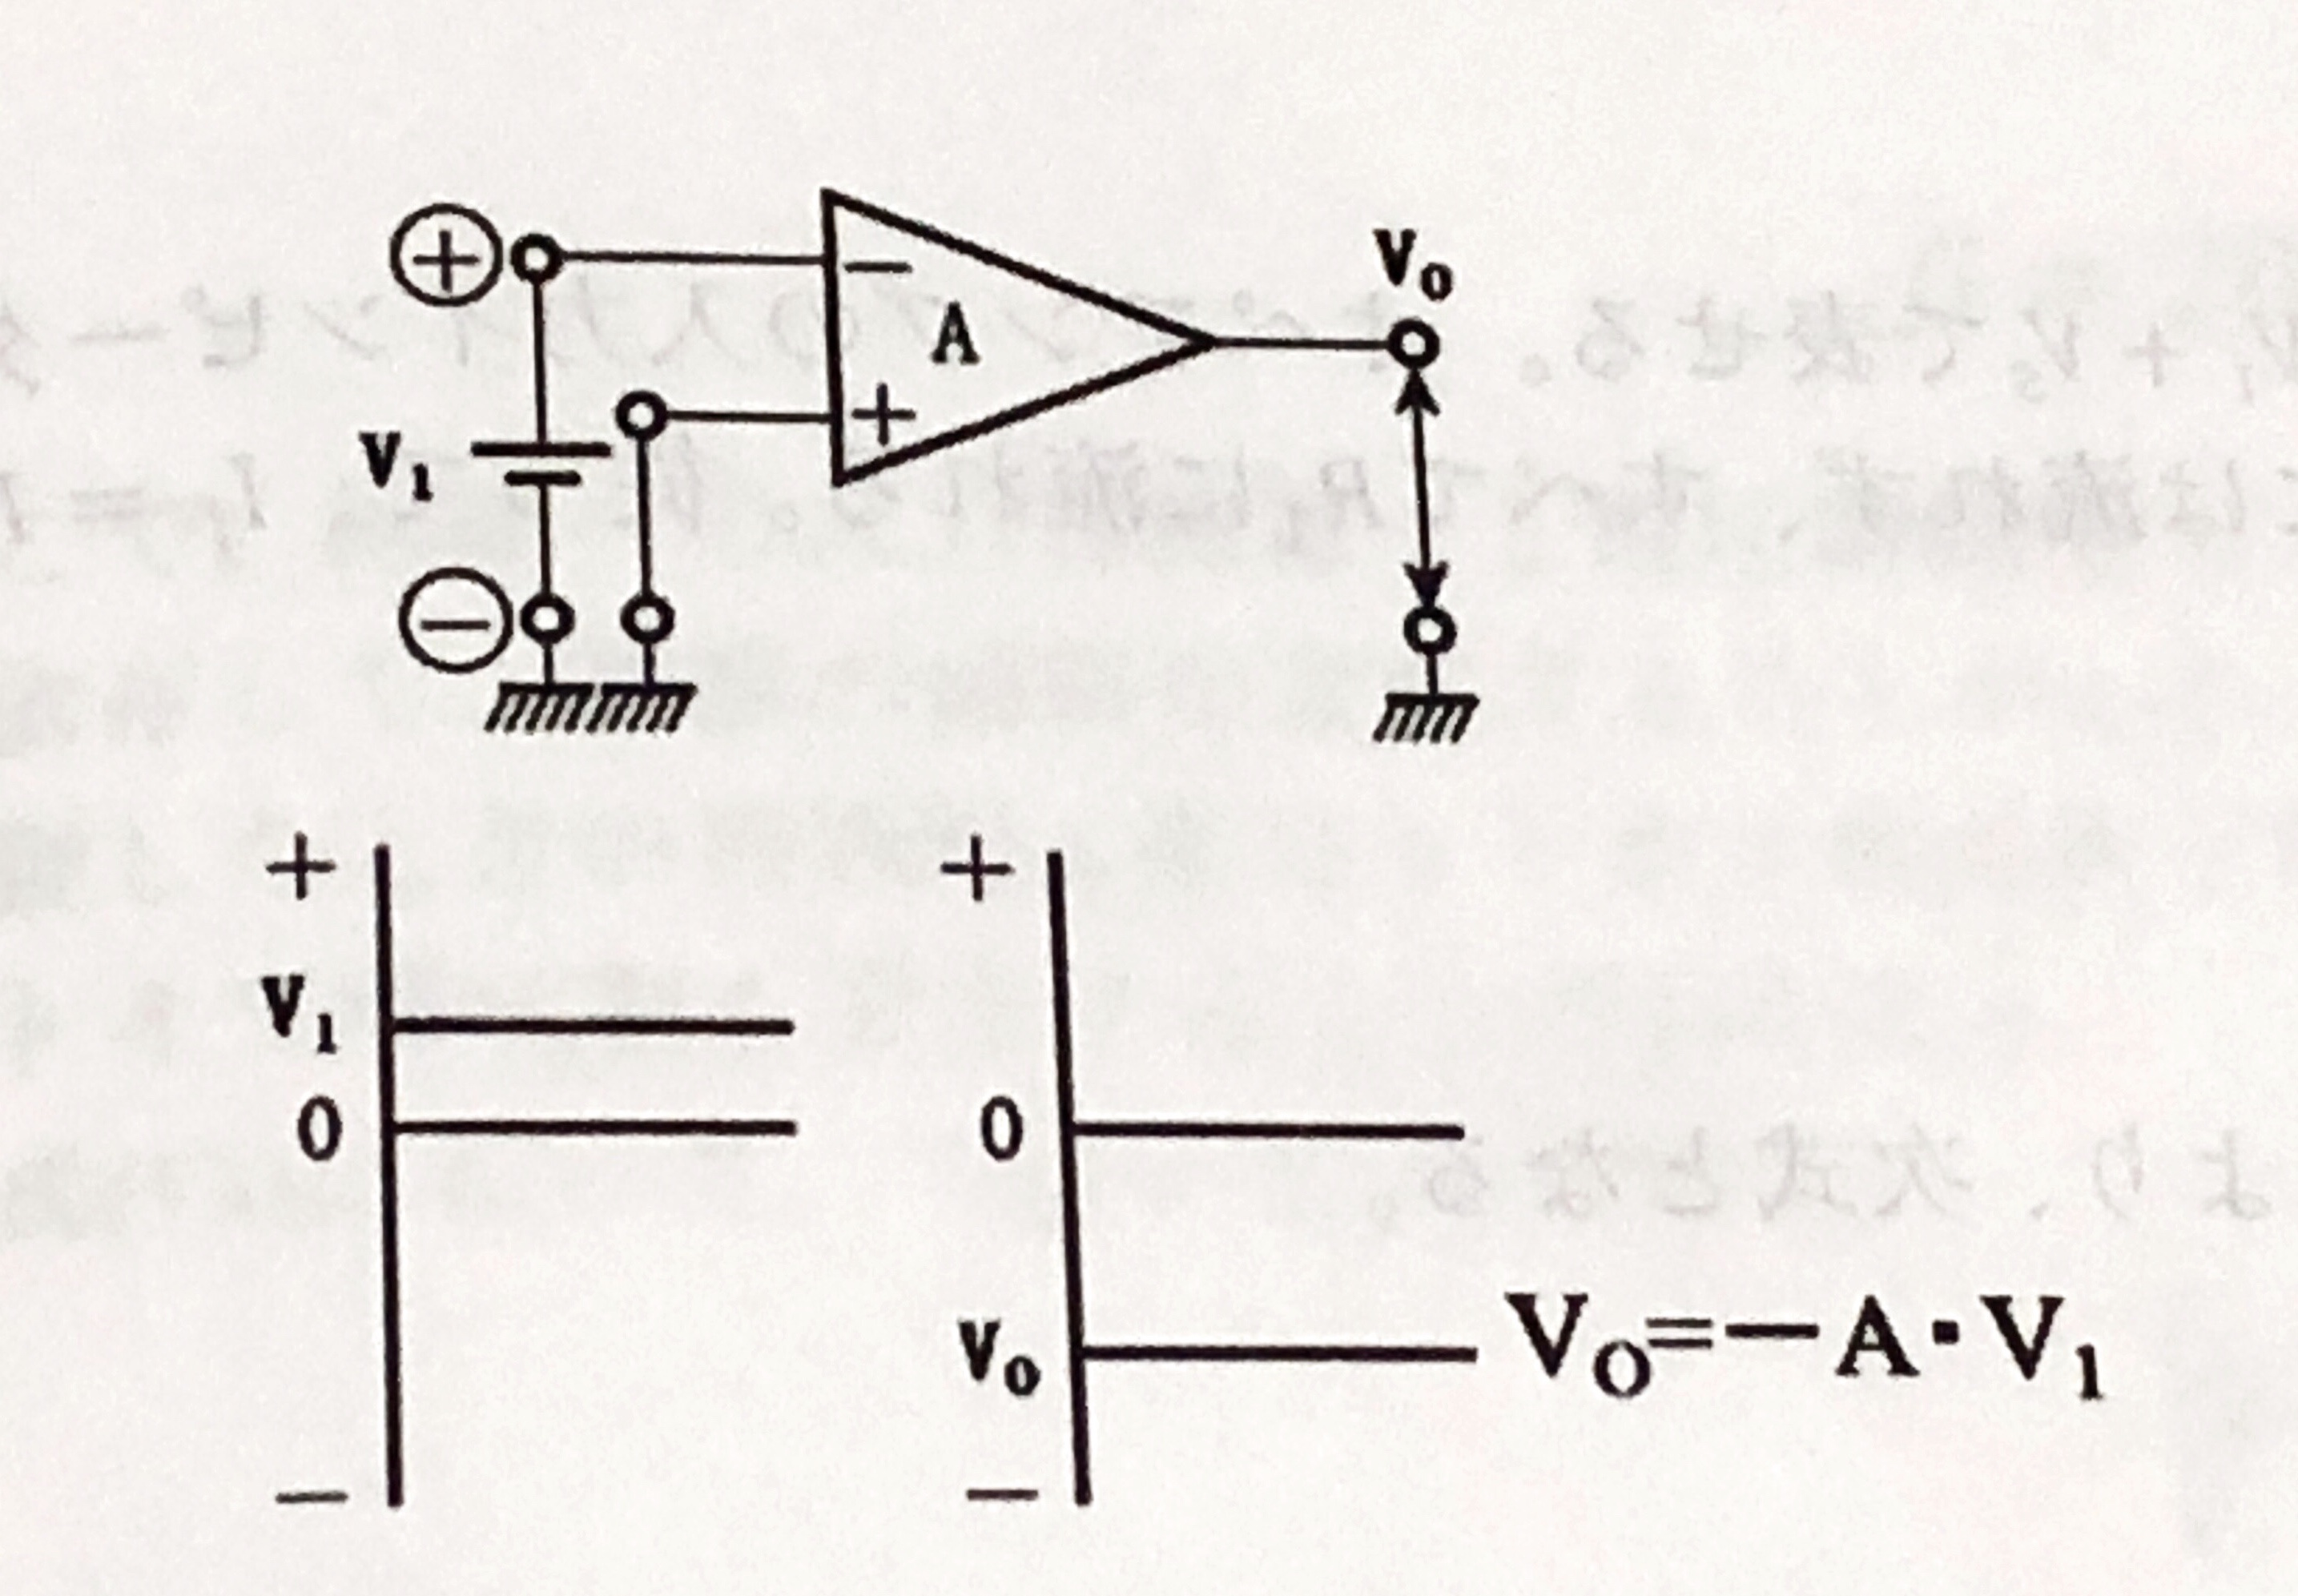
\includegraphics[width=8cm]{画像/addV1.jpg}
		\caption{反転入力に$V_1$を加えた場合}
		\label{addV1}
	\end{center}

\end{figure}
\begin{figure}[H]
	\begin{center}
		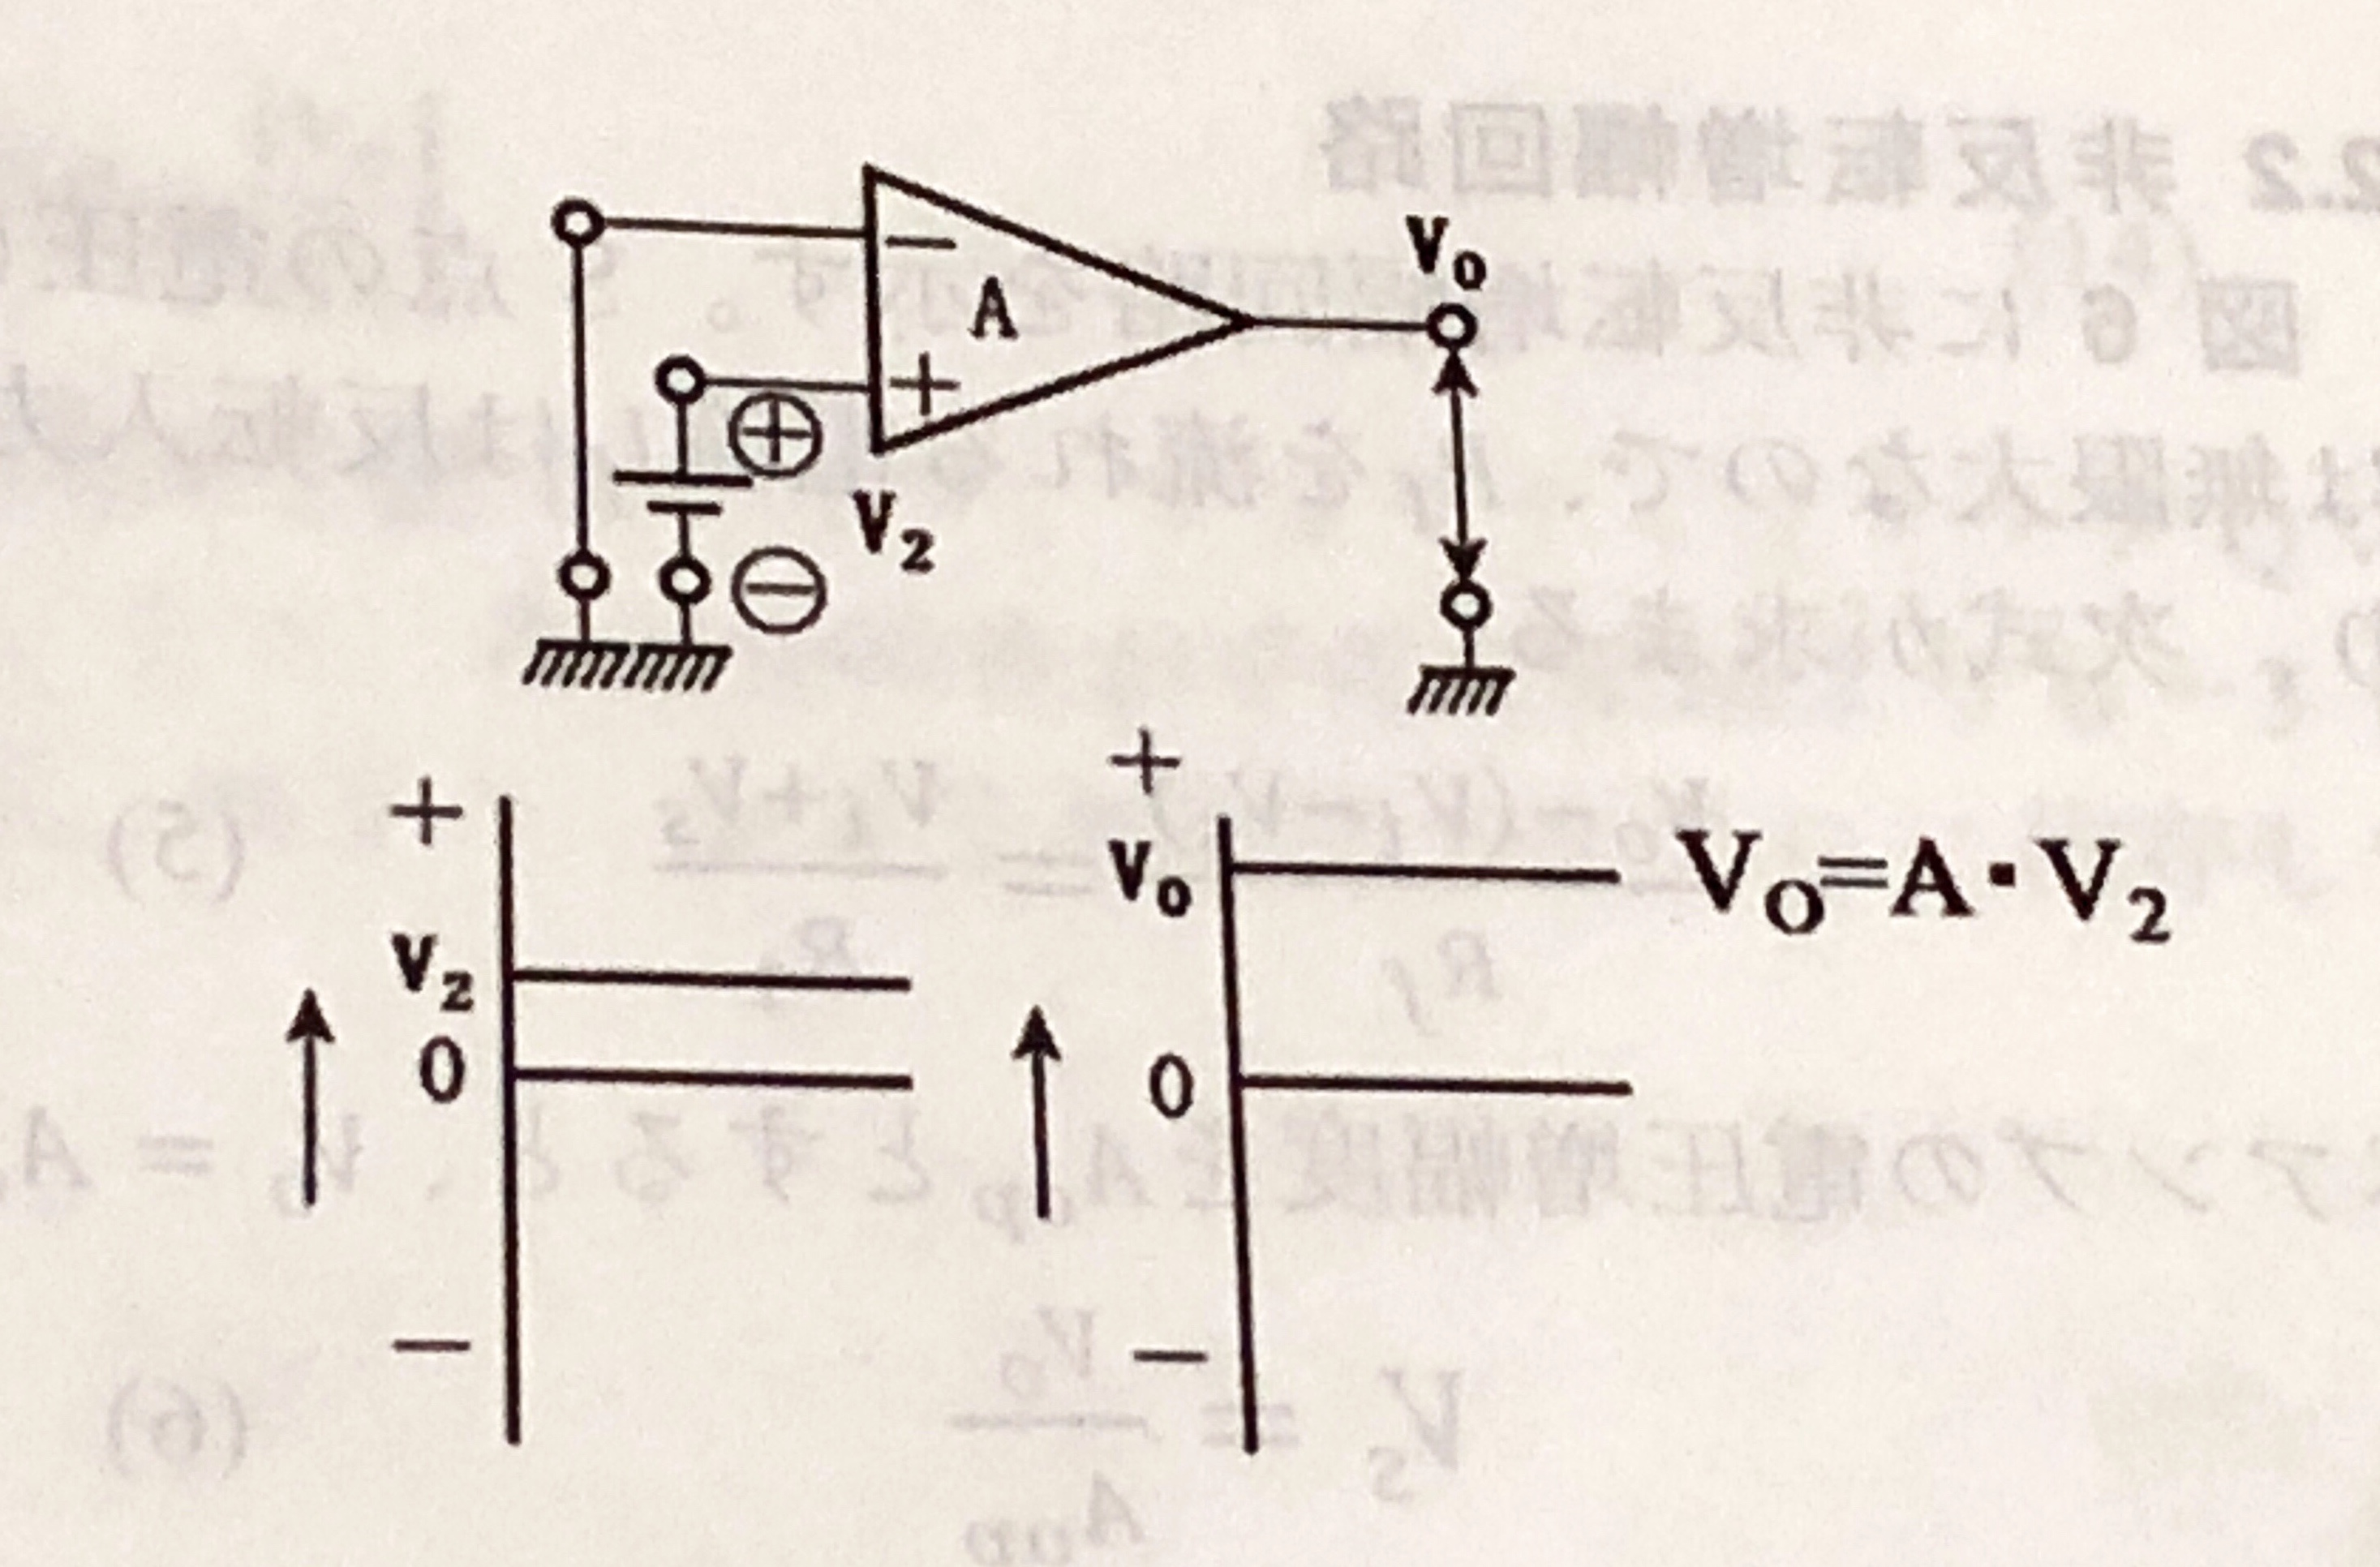
\includegraphics[width=8cm]{画像/addV2.jpg}
		\caption{非反転入力に$V_2$を加えた場合}
		\label{addV2}
	\end{center}
\end{figure}

\subsubsection{反転増幅回路}
\begin{figure}[H]
	\begin{center}
		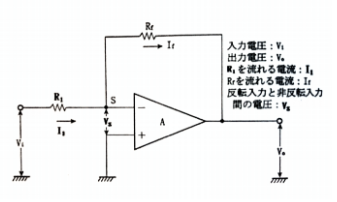
\includegraphics[width=8cm]{画像/反転増幅回路.png}
		\caption{反転増幅回路}
		\label{反転増幅回路}
	\end{center}
\end{figure}

図\ref{反転増幅回路}に反転増幅回路を示す。オペアンプの入力インピーダンスは無限大であるから、$R_1$を流れる電流$I_1$は反転入力には流れず、全て$R_f$に流れる。
すると、$I_1 = I_f$となり、次の式が成り立つ。
\begin{align}
  \frac{V_i-V_s}{R_1} = \frac{V_s-V_0}{R_f}
\end{align}
オペアンプの電圧増幅度を$A_{0p}$とすると、$V_0 = -A_{0p}V_s$から次式のようになる。
\begin{align}
  V_s = -\frac{V_0}{A_{0p}}
\end{align}
理想的には$A_{0p}$は無限大なので、$V_s = 0$となり、非反転入力の電圧と等しくなる。$V_s = 0$として電圧増幅度$A$を考える。
電圧増幅度は,
\begin{align}
  A = \frac{V_0}{V_i}
\end{align}
となり、入力電圧$V_i$はオームの法則により、$V_i = I_1R_1$とすると、$V_0 = -I_1R_f$であるから、
\begin{align}
  A = -\frac{R_f}{R_1}
\end{align}
となる。したがって、反転増幅回路の電圧増幅度$A$は$R_f$と$R_1$によって決定され、入力に対して出力は極性が逆になる。

\subsubsection{非反転増幅回路}
\begin{figure}[H]
	\begin{center}
		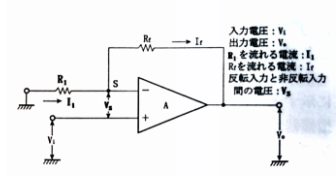
\includegraphics[width=8cm]{画像/非反転増幅回路.png}
		\caption{非反転増幅回路}
		\label{非反転増幅回路}
	\end{center}
\end{figure}

図\ref{非反転増幅回路}に非反転増幅回路を示す。点Sでの電圧は$V_i+V_s$. オペアンプの入力インピーダンスは無限大なので、$R_f$を流れる電流$I_f$は全て$R_1$に流れる。
したがって$I_f=I_1$となり、次式が成り立つ。
\begin{align}
  \frac{V_0 - (V_i - V_s)}{R_f} = \frac{V_i + V_s}{R_1}
\end{align}
オペアンプの電圧増幅度$A_op$とすると、$V_0 = A_opV_s$から、次式となる。
\begin{align}
  V_s = \frac{Vo}{A_op}
\end{align}
理想的には$A_op$は無限大なので$V_s = 0$となり、非反転入力の電圧と等しくなる。$V_s = 0$として電圧増幅度$A$を考えると、
\begin{align}
  \label{7式}
  A = \frac{V_0}{V_i}
\end{align}
$V_s = 0$とすると、次式が得られる。
\begin{align}
  \label{8式}
  \frac{V_0-V_i}{R_f} = \frac{V_i}{R_1}
\end{align}
(\ref{7式})式、(\ref{8式})式より、
\begin{align}
  A = 1 + \frac{R_f}{R_1}
\end{align}
よって、非反転増幅回路の電圧増幅度$A$は$R_f$と$R_1$によって決定され、入力に対しては極性が等しくなる。

\subsubsection{アクティブフィルタ}

\begin{figure}[H]
	\begin{center}
		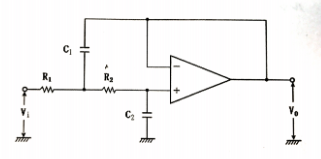
\includegraphics[width=8cm]{画像/アクティブフィルタ.png}
		\caption{ローパスフィルタの基本回路}
		\label{アクティブフィルタ}
	\end{center}
\end{figure}

図\ref{アクティブフィルタ}にオペアンプを用いたローパスフィルタの回路図を示す。入力電圧を$V_i$、出力電圧を$V_0$としたときの入出力電圧の関係は、
\begin{align}
  \label{式10}
  \frac{V_0}{V_i} = \frac{\frac{1}{R_1R_2C_1C_2}}{S^2 + \frac{S}{C_1} \left(\frac{R_1 + R_2}{R_1R_2} \right) + \frac{1}{R_1R_2C_1C_2}}
\end{align}
\begin{align}
  \left(S=j\omega, \omega=2\pi f\right) \nonumber
\end{align}
という式で表される。ここで、クオリティファクタをQとおくと、
\begin{align}
  \omega_0 = \frac{1}{\sqrt{R_1R_2C_1C_2}} \left(f_0=\frac{1}{2\pi \sqrt{R_1R_2C_1C_2}}\right)
\end{align}
\begin{align}
  Q = \frac{1}{R_1 + R_2}\sqrt{\frac{C_1R_1R_2}{C_2}}
\end{align}
式(\ref{式10})は以下のように表すことができる。
\begin{align}
	\label{式13}
  \frac{V_0}{V_i} = \frac{\omega_0^2}{S^2 + \frac{\omega_0}{Q}S + \omega_0^2}
\end{align}

また、$R_1$と$C_1$及び、$R_2$と$C_2$をそれぞれ置き換えると、入出力関係は以下の式で表されるハイパスフィルタとなる。
\begin{align}
	\label{式14}
  \frac{V_0}{V_i} = \frac{S^2}{S^2 + \frac{S}{R_2}\left(\frac{C_1+C_2}{C_1C_2}\right) + \frac{1}{R_1R_2C_1C_2}}
  =\frac{S^2}{S^2+\frac{\omega_0}{Q}S +\omega_0}
\end{align}
\begin{align}
  \omega_0 = \frac{1}{\sqrt{R_1R_2C_1C_2}}, Q = \frac{1}{C_1 + C_2}\sqrt{\frac{C_1C_1R_2}{R_1}}
\end{align}

\subsubsection{微分回路}
\begin{figure}[H]
	\begin{center}
		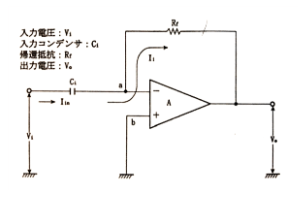
\includegraphics[width=8cm]{画像/微分回路.png}
		\caption{微分回路}
		\label{微分回路}
	\end{center}
\end{figure}

図\ref{微分回路}に微分回路を示す。
$C_i$を流れる電流を$Ii$とすると、a点の電圧はb点の電圧と等しいので、$V_0$は以下のようになる。
\begin{align}
  V_0 = -I_iR_f = -C_iR_f \frac{\mathrm{d} V_i}{\mathrm{d} t}
\end{align}
このように、$V_0$は、入力電圧$V_i$を微分した値に比例する出力となる。
微分器として安定な上限の周波数$f_s$は次式で求まる。
\begin{align}
  f_s = \frac{1}{2\pi R_iC_i}
\end{align}

\subsubsection{積分回路}

\begin{figure}[H]
	\begin{center}
		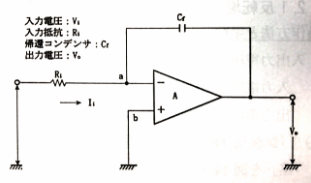
\includegraphics[width=8cm]{画像/積分回路.png}
		\caption{積分回路}
		\label{積分回路}
	\end{center}
\end{figure}

図\ref{積分回路}に積分回路を示す。
$R_i$を流れる電流を$Ii$とすると、a点の電圧はb点の電圧と等しいので、以下の式が成り立つ。
\begin{align}
  \frac{\mathrm{d}Q_f}{\mathrm{d}t} = I_i
\end{align}
これを積分すると、
\begin{align}
  Q_f = \int I_i \mathrm{d}t = \frac{1}{R_i}\int V_i \mathrm{d}t
\end{align}
となる。$V_0$はコンデンサ$C_f$による電圧降下量$-Q_f/C_f$に等しいので、
\begin{align}
  V_0 = -\frac{1}{R_iC_f}\int V_i\mathrm{d}t
\end{align}
となり、入力電圧$V_i$を積分した値に比例する出力が得られることになる。
積分器として安定な下限の周波数$f_p$は次式で求まる。
\begin{align}
  f_p = \frac{1}{2\pi R_fC_f}
\end{align}

\section{実験方法}
\subsection{反転増幅回路の入出力特性}
\begin{enumerate}
  \item 回路を図\ref{A=-1}のように組み、反転増幅回路を作成した。
  \item 試験用DC電圧発生部の-3V〜+3Vボリュームで入力電圧を0Vに調整した。
  \item 出力電圧が0Vであることをオシロスコープで確認した。
  \item 試験用DC電圧を-3V〜+3Vまで0.5V間隔で変え、入出力電圧をオシロスコープで観測した。
  \item 入力電圧と出力電圧の表を作成し、グラフにした。
  \item $A=−10$となるような回路(図\ref{A=-10})を作成した。
  \item 5., 6.の同様の操作を行った。
\end{enumerate}

\begin{figure}[H]
	\begin{center}
		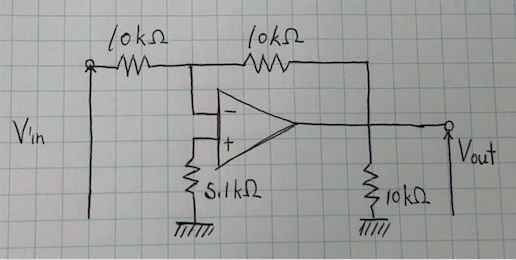
\includegraphics[width=8cm]{画像/A=-1.png}
		\caption{$A=-1$となる反転増幅回路}
		\label{A=-1}
	\end{center}
\end{figure}

\begin{figure}[H]
	\begin{center}
		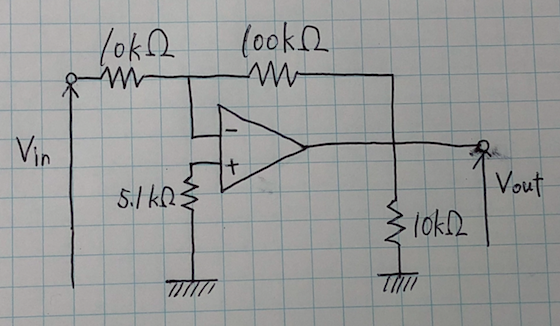
\includegraphics[width=8cm]{画像/A=-10.png}
		\caption{$A=-10$となる反転増幅回路}
		\label{A=-10}
	\end{center}
\end{figure}

\subsection{反転増幅回路の周波数特性及び位相}
\begin{enumerate}
  \item 試験用DC電圧発生部の接続を外し、信号発生器を接続した。
  \item オシロスコープを$V_{in}$及び$V_{out}$に接続した。
  \item 信号発生器の出力を1.2$\mathrm{V_{p-p}}$, 100Hzに設定した。
  \item 周波数を100Hzから1MHzまで変えた。この際、出力電圧の振幅と位相の変化をオシロスコープで観察し、低周波では入出力は系の位相差が180度であることをオシロスコープで確認した。
  \item 4.のデータから周波数$f$,電圧増幅度$G$の関係をグラフにした。
\end{enumerate}

\subsection{ローパスフィルタ回路}
\begin{figure}[H]
	\begin{center}
		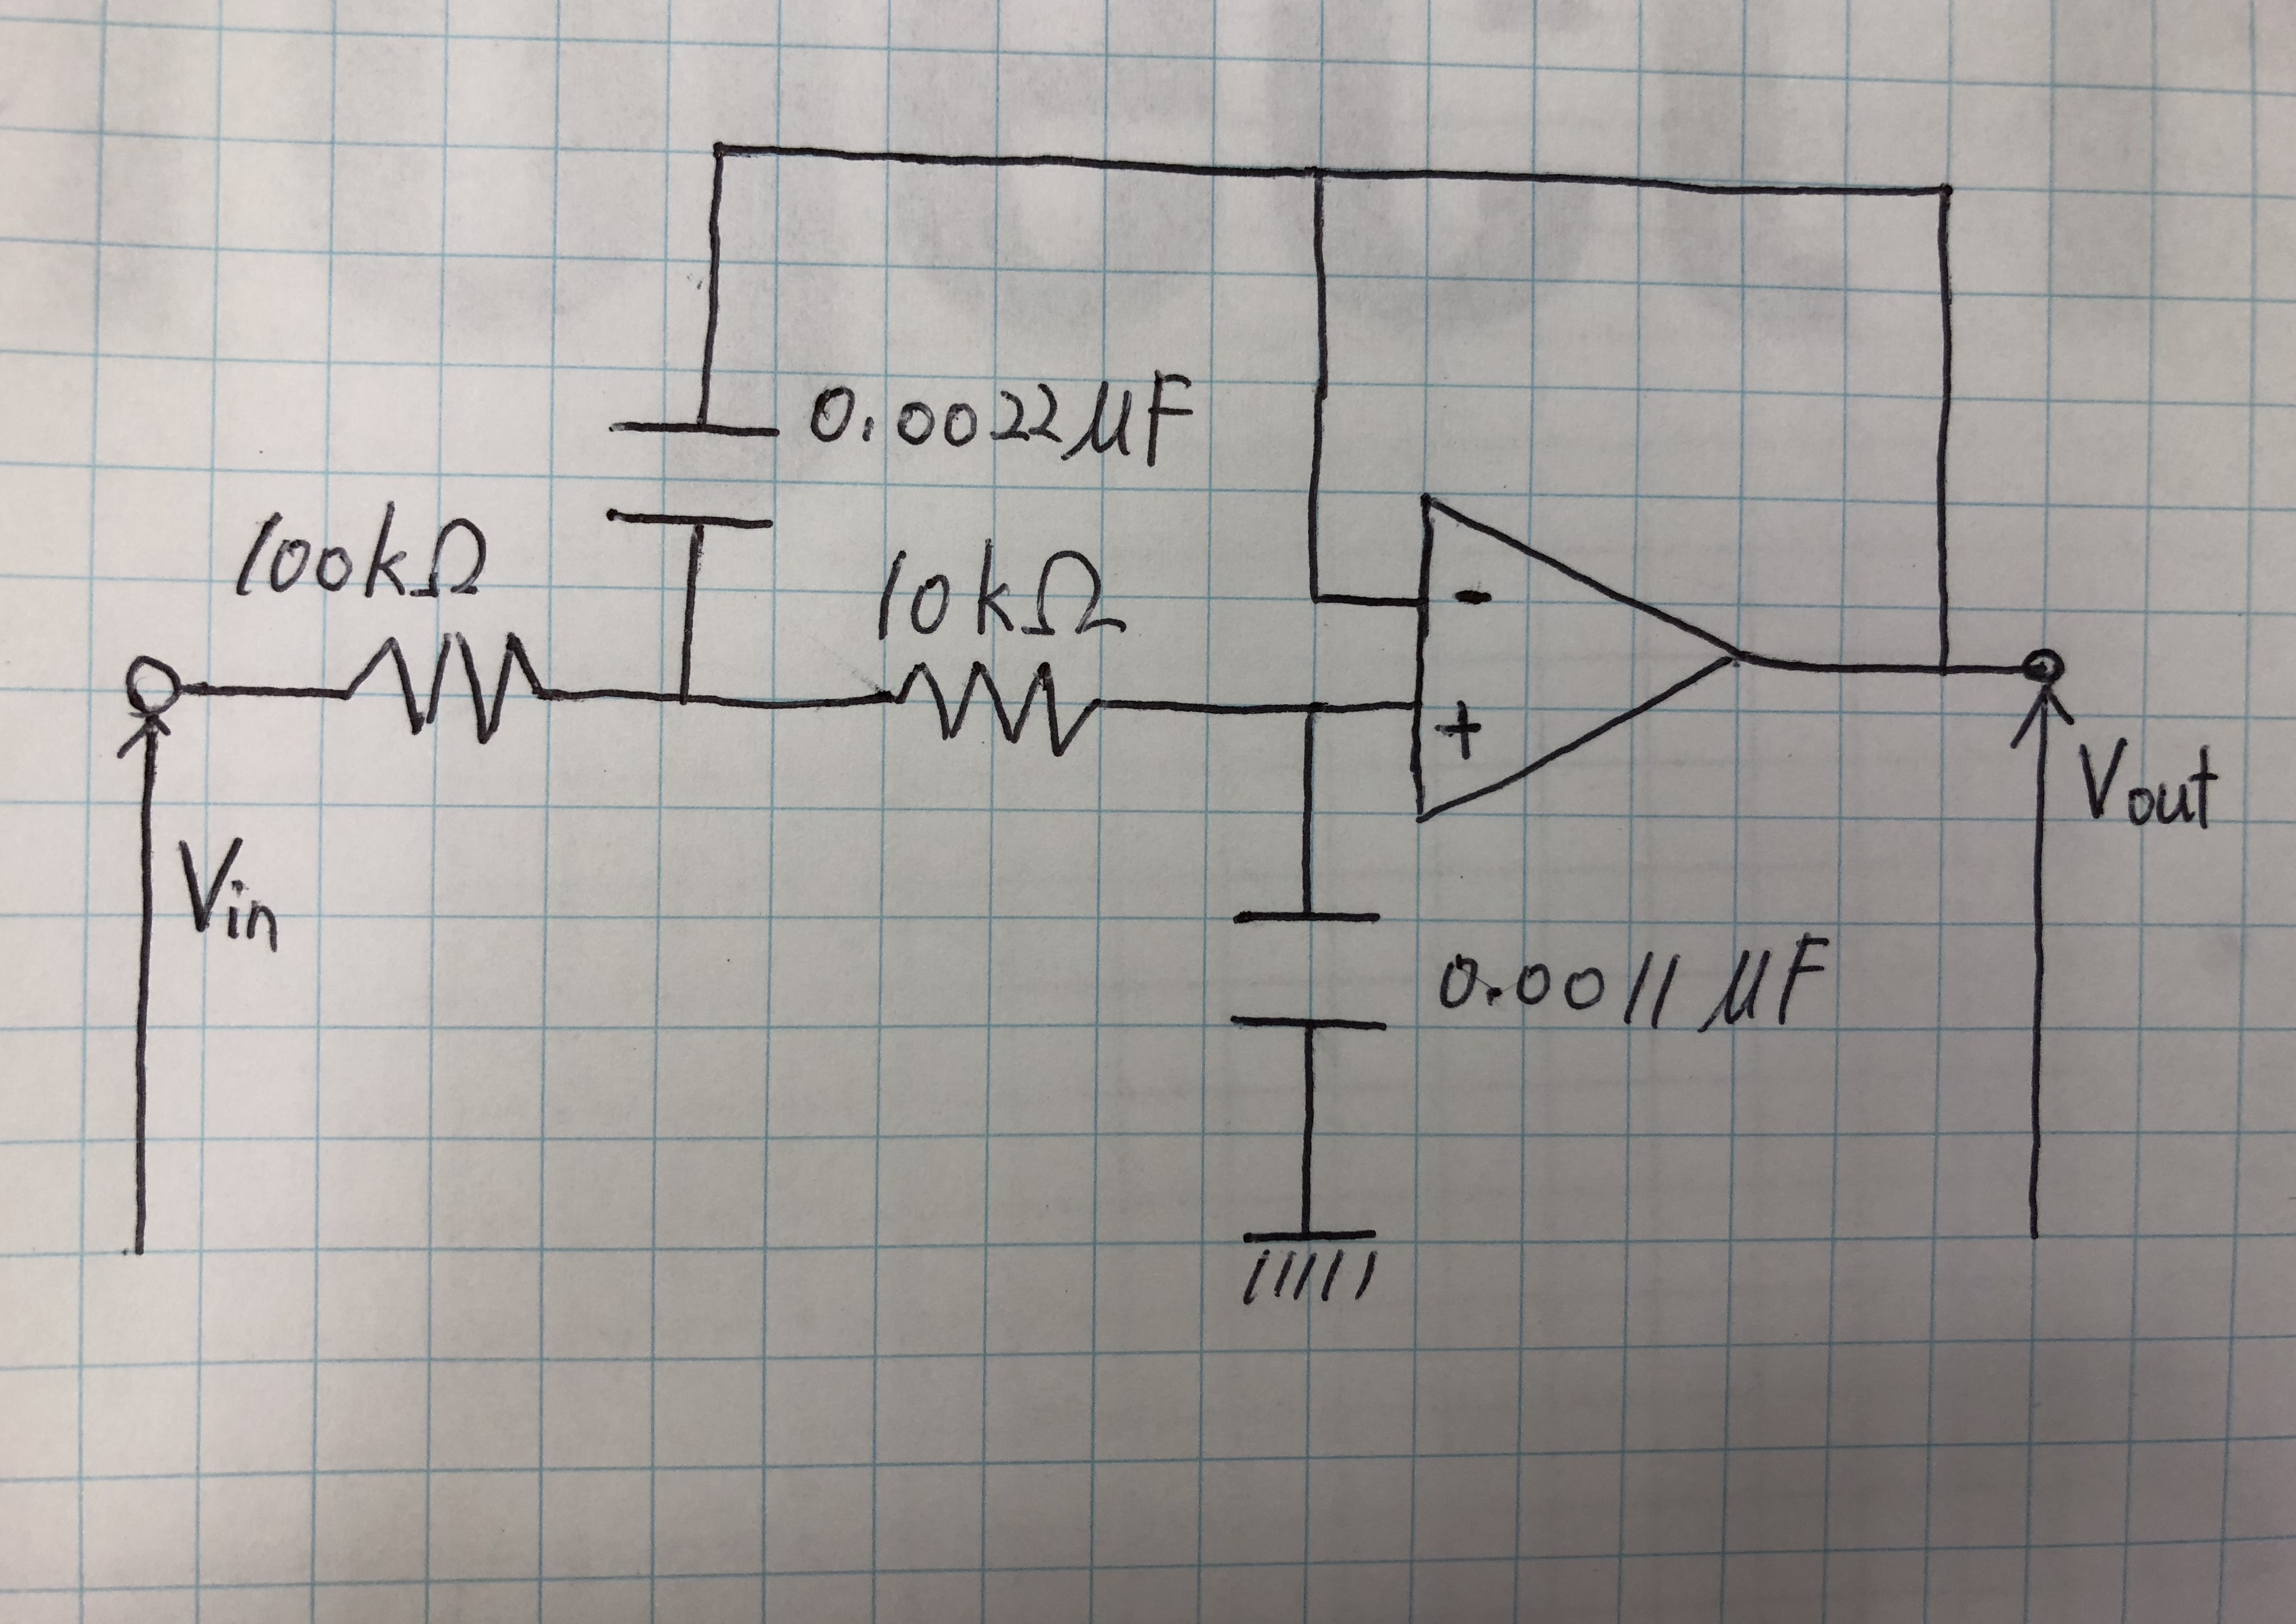
\includegraphics[width=8cm]{画像/ローパス1.jpg}
		\caption{ローパスフィルタ回路図}
		\label{ローパスフィルタ}
	\end{center}
\end{figure}

\begin{enumerate}
  \item 図\ref{ローパスフィルタ}のようなローパスフィルタをを作成した。
  \item 作成した回路の$Q$及び$\omega_0,f_0$を計算により求めた。
  \item 信号発生器の出力を1.2$\mathrm{V_{p-p}}$に設定し、10kHzの方形波を入力し、出力波形を観察した。
  \item $f_0$を含む20パターン程度の周波数の正弦波を入力し、入力電圧及び出力電圧を計測した。
  \item 電圧増幅度$G$に換算して、$f-G$特性をグラフにした。
\end{enumerate}

\subsection{ハイパスフィルタ回路}
\begin{figure}[H]
	\begin{center}
		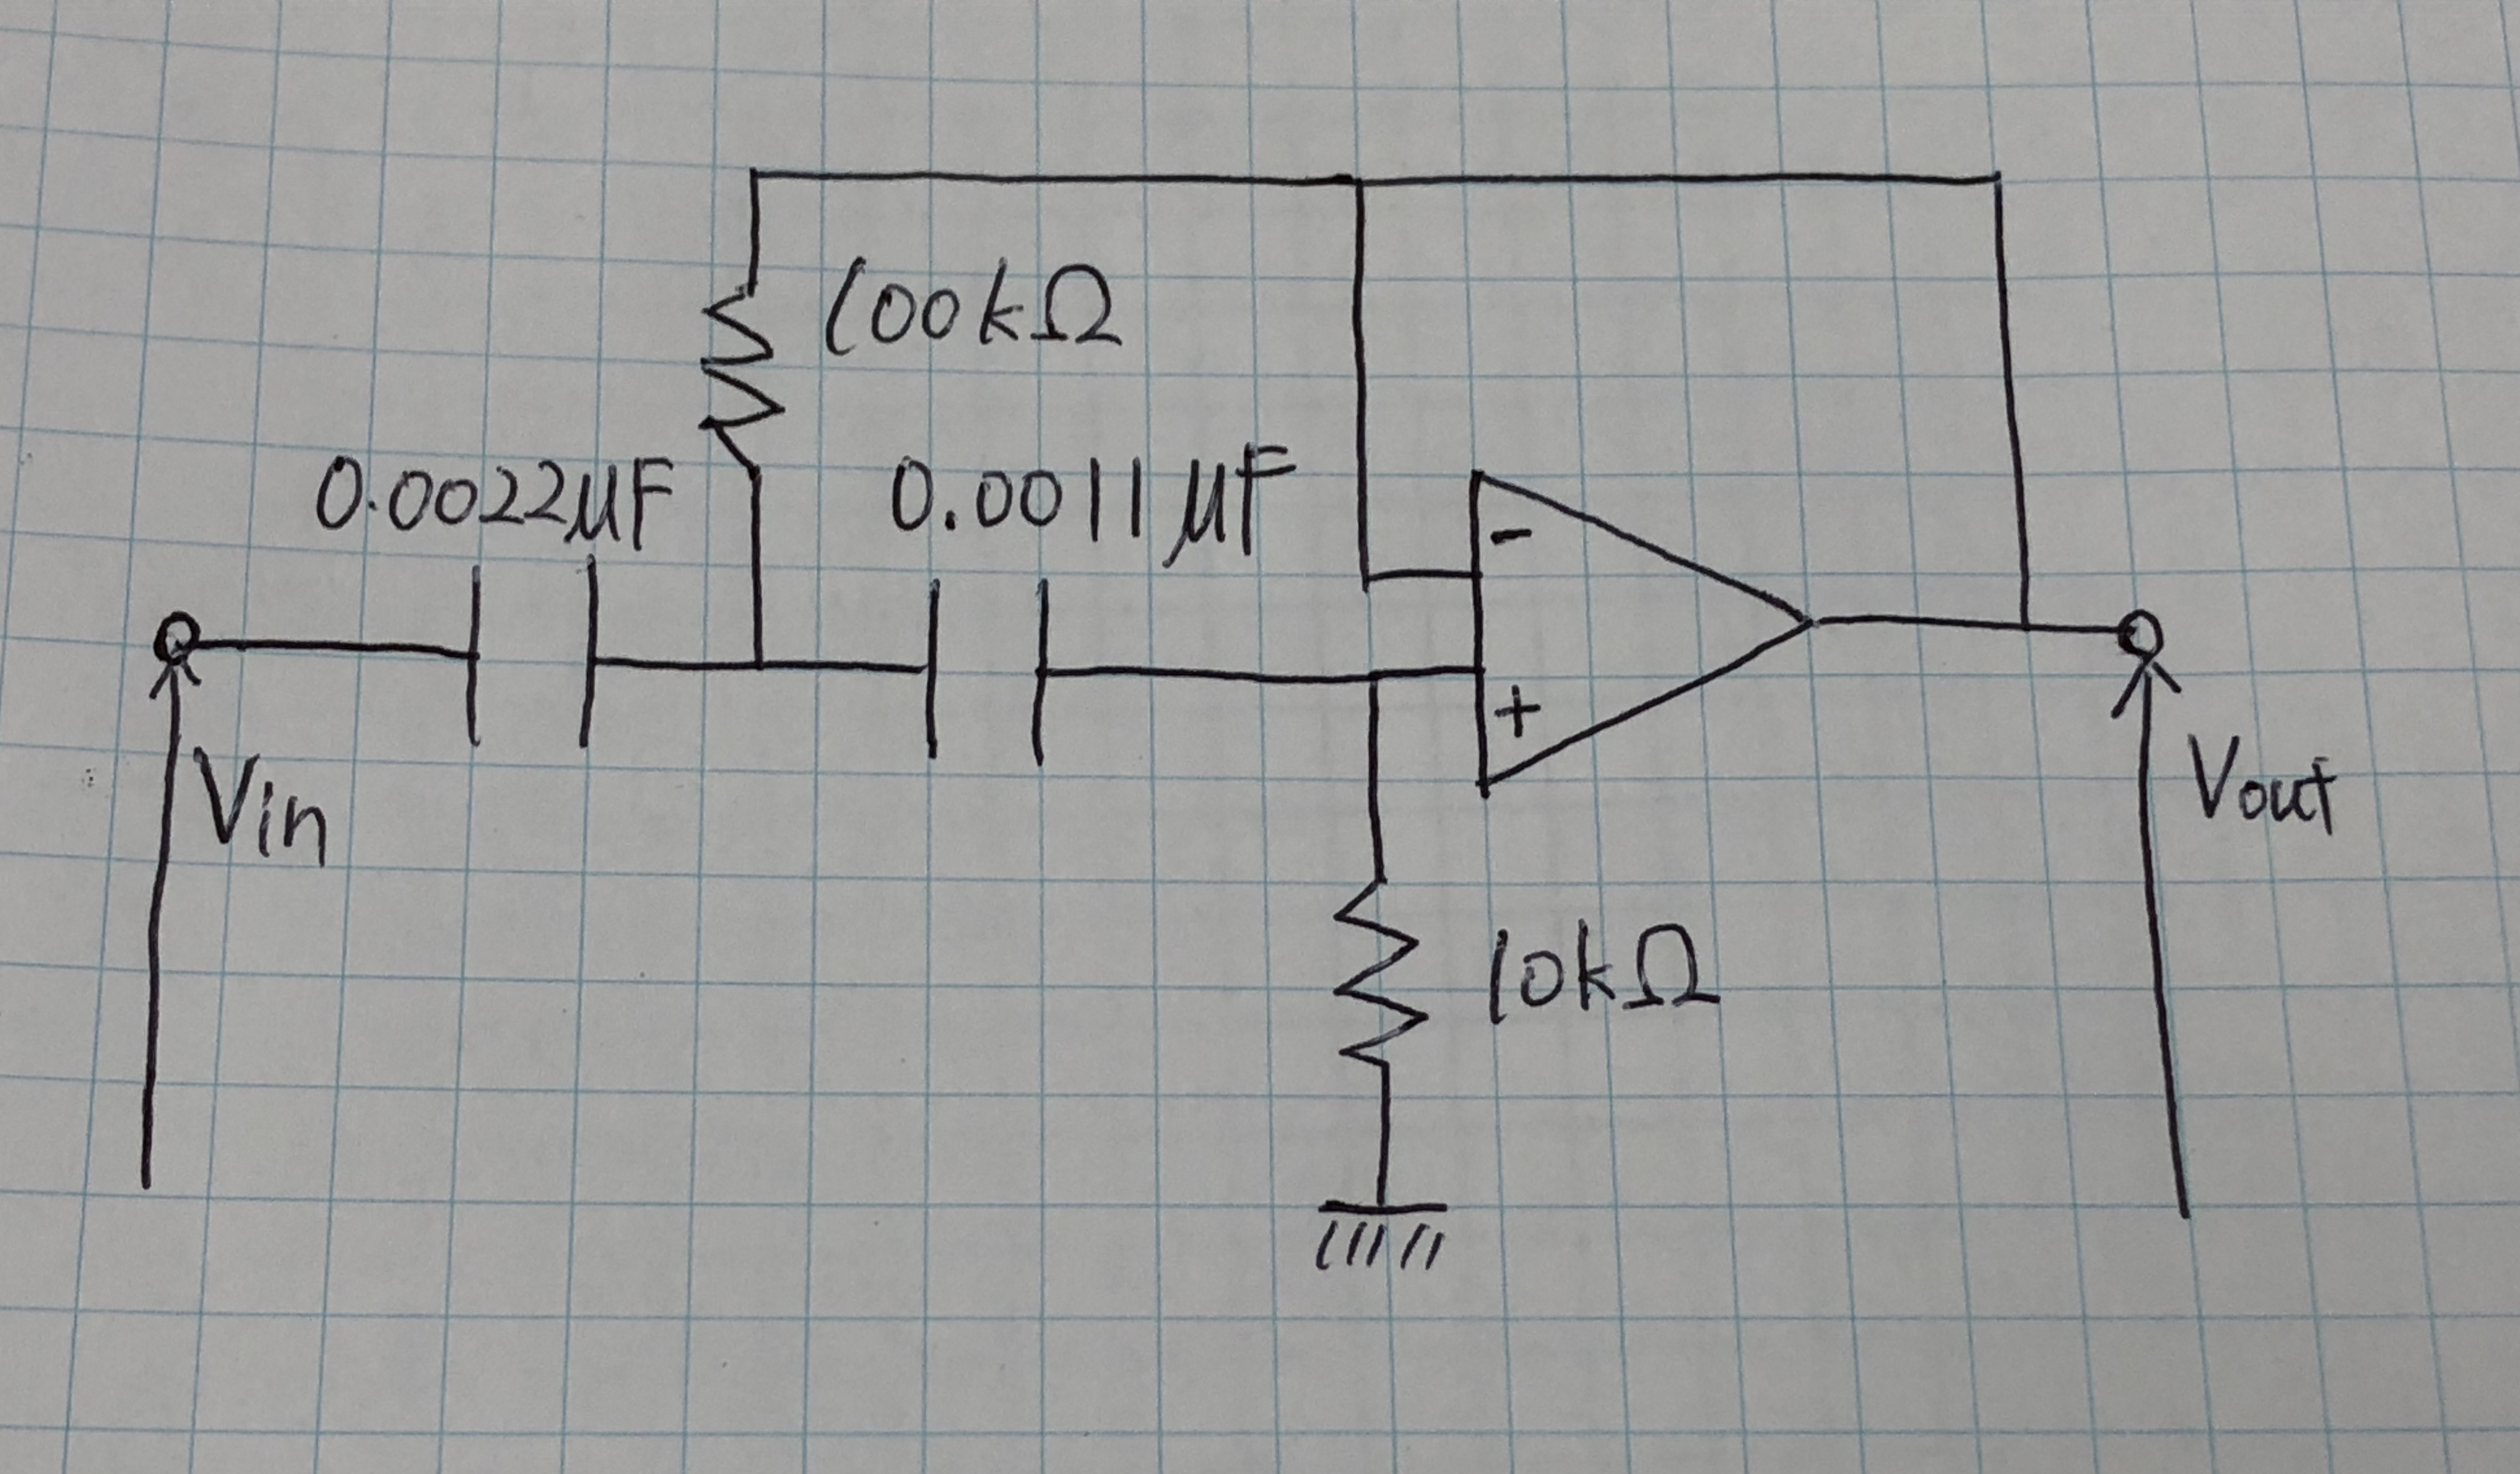
\includegraphics[width=8cm]{画像/ハイパス1.jpg}
		\caption{ハイパスフィルタ回路図}
		\label{ハイパスフィルタ}
	\end{center}
\end{figure}

\begin{enumerate}
  \item 図\ref{ハイパスフィルタ}のようなハイパスフィルタをを作成した。
  \item 作成した回路の$Q$及び$\omega_0,f_0$を計算により求めた。
  \item 信号発生器の出力を1.2$\mathrm{V_{p-p}}$に設定し、10kHZの方形波を入力し、出力波形を観察した。
  \item $f_0$を含む20パターン程度の周波数の正弦波を入力し、入力電圧及び出力電圧を計測した。
  \item 電圧増幅度$G$に換算して、$f-G$特性をグラフにした。
\end{enumerate}

\subsection{微分回路}
\begin{figure}[H]
	\begin{center}
		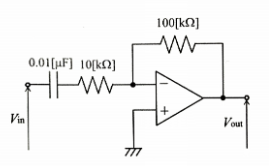
\includegraphics[width=8cm]{画像/微分回路1.png}
		\caption{微分回路の回路図}
		\label{微分回路1}
	\end{center}
\end{figure}

\begin{enumerate}
  \item 図\ref{微分回路1}のような微分回路を作成した。
  \item 微分器として安定な上限の周波数$f_s$を計算により求めた。
  \item 信号発生器の出力を1$\mathrm{V_{p-p}}$の方形波に設定し、$f=f_s,f>f_s,f<f_s$の3通りの出力波形を観察した。
\end{enumerate}

\subsection{積分回路}
\begin{figure}[H]
	\begin{center}
		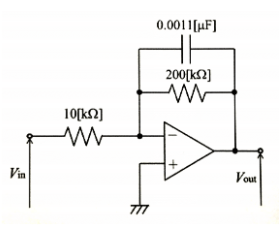
\includegraphics[width=8cm]{画像/積分回路1.png}
		\caption{積分回路の回路図}
		\label{積分回路1}
	\end{center}
\end{figure}

\begin{enumerate}
  \item 図\ref{積分回路1}のような積分回路を作成した。
  \item 積分器として安定な上限の周波数$f_p$を計算により求めた。
  \item 信号発生器の出力を1$\mathrm{V_{p-p}}$の方形波に設定し、$f=f_p,f>f_p,f<f_p$の3通りの出力波形を観察した。
\end{enumerate}

\section{結果}
\subsection{反転増幅回路の入出力特性}
反転増幅回路($A = -1,-10$)の入出力特性をそれぞれ表\ref{A=-1表},図\ref{入出力電圧1}と表\ref{A=-10表}, 図\ref{入出力電圧2}に示した。
なお、$A=-1$では近似直線$-0.683x + 0.0141$を引いてある.
$A=-1$の場合では, -3V〜3Vまで入力電圧が上がるにつれ, 出力電圧が2V〜-2Vまで低下している.
$A=-10$の場合では, 入力電圧が約1.5V以上, また約-1.5V以下までは出力電圧が一定であり,
入力電圧が-1.5V〜1.5Vの範囲では上がるにつれ, 出力電圧が14.5V〜-12.5Vまで低下していることがわかる.
\begin{table}[H]
	\caption{$A=-1$における入出力電圧の関係}
	\label{A=-1表}
	\begin{center}
    \begin{tabular}[H]{|c|c|}\hline
      入力電圧[$\mathrm{V_{p-p}}$] & 出力電圧[$\mathrm{V_{p-p}}$] \\ \hline
      3 & -2.01 \\ \hline
      2.47 & -1.63 \\ \hline
      2.05 & -1.32 \\ \hline
      1.48 & -0.945 \\ \hline
      1 & -0.614 \\ \hline
      0.52 & -0.286 \\ \hline
      0.0028 & -0.0594 \\ \hline
      -0.525 & 0.413 \\ \hline
      -0.995 & 0.73 \\ \hline
      -1.53 & 1.09 \\ \hline
      -2 & 1.4 \\ \hline
      -2.5 & 1.7 \\ \hline
      -2.95 & 1.7 \\ \hline
    \end{tabular}
\end{center}
\end{table}

\begin{figure}[H]
	\begin{center}
		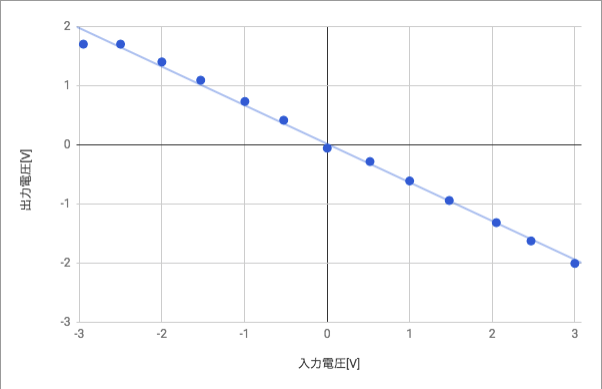
\includegraphics[width=8cm]{画像/A=-1入出力.png}
		\caption{$A=-1$における入出力電圧の関係}
		\label{入出力電圧1}
	\end{center}
\end{figure}

\begin{table}[H]
	\caption{$A=-10$における入出力電圧の関係}
	\label{A=-10表}
	\begin{center}
    \begin{tabular}[H]{|c|c|}\hline
      入力電圧[$\mathrm{V_{p-p}}$] & 出力電圧[$\mathrm{V_{p-p}}$] \\ \hline
      2.97 & -12.5 \\ \hline
      2.49 & -12.5 \\ \hline
      2.01 & -12.5 \\ \hline
      1.52 & -12.5 \\ \hline
      0.996 & -8.85 \\ \hline
      0.502 & -3.93 \\ \hline
      -0.00365 & 1.1 \\ \hline
      -0.507 & 6.01 \\ \hline
      -1.03 & 11.2 \\ \hline
      -1.53 & 14.6 \\ \hline
      -2.01 & 14.5 \\ \hline
      -2.52 & 14.5 \\ \hline
      -2.96 & 14.5 \\ \hline
    \end{tabular}
\end{center}
\end{table}

\begin{figure}[H]
	\begin{center}
		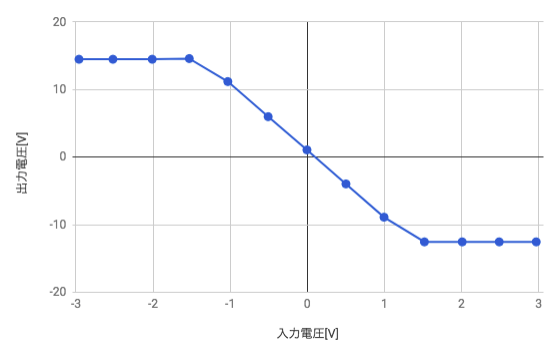
\includegraphics[width=8cm]{画像/A=-10入出力.png}
		\caption{$A=-10$における入出力電圧の関係}
		\label{入出力電圧2}
	\end{center}
\end{figure}

\subsection{反転増幅回路の周波数特性及び位相}
出力電圧の振幅と位相の変化は表\ref{周波数特性}のようになった。また、周波数$f$と電圧増幅度$G$を片対数グラフとして図\ref{片対数1}に示した。
周波数が30kHzから電圧増幅度の低下が始まり, 1000kHzまでおおよそ直線的に電圧増幅度が低下している.

\begin{table}[H]
	\caption{反転増幅回路の周波数特性及び位相}
	\label{周波数特性}
	\begin{center}
    \begin{tabular}[H]{|c|c|c|c|c|c|}\hline
      周波数[kHz] & 入力電圧$V_{in}$[Vp-p] & 出力電圧$V_{out}$[Vp-p] & 位相差[s] & 位相差[度] & 電圧増幅度$G$[dB] \\ \hline
      0.1 & 1.2 & 12 & 0.005 & 180 & 20 \\ \hline
      0.5 & 1.2 & 12 & 0.001 & 180 & 20 \\ \hline
      1 & 1.2 & 12.2 & 0.0005 & 180 & 20.14357169 \\ \hline
      5 & 1.24 & 12.6 & 0.0001 & 180 & 20.1389772 \\ \hline
      10 & 1.2 & 12.2 & 0.000052 & 187.2 & 20.14357169 \\ \hline
      20 & 1.22 & 12 & 0.000027 & 194.4 & 19.85642831 \\ \hline
      30 & 1.22 & 11.6 & 0.0000188 & 203.04 & 19.56196317 \\ \hline
      40 & 1.22 & 10.8 & 0.0000148 & 213.12 & 18.9412785 \\ \hline
      50 & 1.22 & 10.2 & 0.000012 & 216 & 18.44480682 \\ \hline
      60 & 1.22 & 9.6 & 0.0000102 & 220.32 & 17.91822805 \\ \hline
      70 & 1.22 & 9 & 0.000009 & 0.2268 & 17.35765358 \\ \hline
      80 & 1.22 & 8.6 & 0.000008 & 230.4 & 16.96277241 \\ \hline
      90 & 1.22 & 8 & 0.0000074 & 239.76 & 16.33460313 \\ \hline
      100 & 1.22 & 7.4 & 0.0000068 & 244.8 & 15.65743778 \\ \hline
      200 & 1.22 & 4.08 & 0.00000352 & 253.44 & 10.48600665 \\ \hline
      300 & 1.24 & 2.96 & 0.00000244 & 263.52 & 7.557400518 \\ \hline
      400 & 1.24 & 2.16 & 0.00000192 & 276.48 & 4.82064132 \\ \hline
      500 & 1.22 & 1.8 & 0.00000156 & 280.8 & 3.378253489 \\ \hline
      600 & 1.22 & 1.48 & 0.00000134 & 289.44 & 1.678037694 \\ \hline
      700 & 1.22 & 1.32 & 0.00000116 & 292.32 & 0.6842820106 \\ \hline
      800 & 1.22 & 1.06 & 0.00000104 & 299.52 & -1.221079308 \\ \hline
      900 & 1.22 & 0.94 & 0.00000094 & 304.56 & -2.264639542 \\ \hline
      1000 & 1.22 & 0.84 & 0.00000088 & 316.8 & -3.241610892 \\ \hline
    \end{tabular}
\end{center}
\end{table}

\begin{figure}[H]
	\begin{center}
		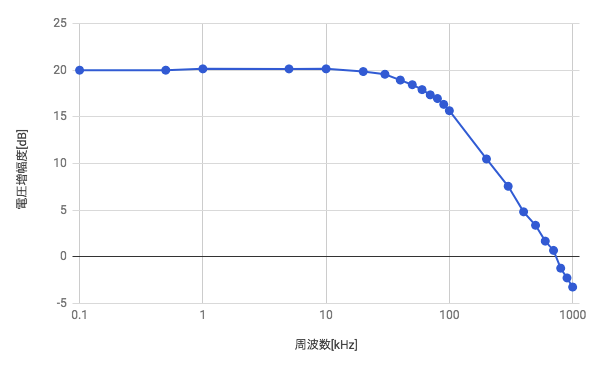
\includegraphics[width=8cm]{画像/片対数1.png}
		\caption{周波数$f$と電圧増幅度$G$を示す片対数グラフ}
		\label{片対数1}
	\end{center}
\end{figure}

\subsection{ローパスフィルタ回路}
回路に用いた抵抗とコンデンサの値と計算値を表\ref{ローパス計算}に示す。
ローパスフィルタの周波数特性は表\ref{ローパス特性}と図\ref{ローパス片対数}のようになった。
また、10kHzの方形波を入力した際の波形を図\ref{ローパス方形波}に示した。
表\ref{ローパス特性}と図\ref{ローパス片対数}を見ると, 300Hz付近から徐々に電圧増幅度の低下が始まり,
1400Hz付近からなだらかに低下していることがわかる. つまり, 低周波数帯では減衰させず、高周波数帯になるにつれ減衰が大きくなる回路であるとわかる.
図\ref{ローパス方形波}の方形波では横線の部分が低周波数で縦線の部分が高周波数となっており、ローパスフィルタを通すことで
波形がなだらかになることがわかる.
\begin{table}[H]
	\caption{ローパスフィルタ回路作成に用いた諸計算値}
	\label{ローパス計算}
	\begin{center}
    \begin{tabular}[H]{|c|c|}\hline
      $R_1$[k$\Omega$] & 100 \\ \hline
      $R_2$[k$\Omega$] & 10\\ \hline
      $C_1$[$\mu$ F] & 0.0022\\ \hline
      $C_2$[$\mu$ F] & 0.0011\\ \hline
      $Q$ & 0.0129 \\ \hline
      $\omega_0$[rad/s] & $2.033 \times 10^4$ \\ \hline
      $f_0$[Hz] & 3235.8\\ \hline
    \end{tabular}
\end{center}
\end{table}

\begin{table}[H]
	\caption{ローパスフィルタにおける周波数特性}
	\label{ローパス特性}
	\begin{center}
    \begin{tabular}[H]{|c|c|c|c|}\hline
      Hz & 入力電圧$V_{in}$[$\mathrm{V_{p-p}}$] & 出力電圧$V_{out}$[$\mathrm{V_{p-p}}$] & 電圧増幅度$G$[dB]  \\ \hline
      50 & 1.2 & 1.2 & 0 \\ \hline
      100 & 1.2 & 1.2 & 0 \\ \hline
      300 & 1.2 & 1.18 & -0.1459847748 \\ \hline
      500 & 1.2 & 1.16 & -0.2944651364 \\ \hline
      600 & 1.2 & 1.14 & -0.4455278942 \\ \hline
      700 & 1.2 & 1.12 & -0.5992644675 \\ \hline
      800 & 1.22 & 1.1 & -0.8993429103 \\ \hline
      900 & 1.22 & 1.08 & -1.058721504 \\ \hline
      1000 & 1.22 & 1.06 & -1.221079308 \\ \hline
      1200 & 1.22 & 1 & -1.727196613 \\ \hline
      1400 & 1.22 & 0.94 & -2.264639542 \\ \hline
      1600 & 1.22 & 0.9 & -2.642346425 \\ \hline
      1800 & 1.22 & 0.84 & -3.241610892 \\ \hline
      2000 & 1.22 & 0.78 & -3.88530456 \\ \hline
      2300 & 1.2 & 0.672 & -5.03623946 \\ \hline
      2500 & 1.2 & 0.66 & -5.19274621 \\ \hline
      2700 & 1.18 & 0.62 & -5.589806356 \\ \hline
      3000 & 1.22 & 0.56 & -6.763436073 \\ \hline
      3235.3 & 1.18 & 0.55 & -6.630386356 \\ \hline
      3500 & 1.2 & 0.51 & -7.432221399 \\ \hline
      4000 & 1.22 & 0.42 & -9.262210806 \\ \hline
      4500 & 1.18 & 0.352 & -10.50678688 \\ \hline
      5000 & 1.2 & 0.32 & -11.48062535 \\ \hline
      6000 & 1.22 & 0.264 & -13.29511808 \\ \hline
      7000 & 1.22 & 0.212 & -15.20047939 \\ \hline
      8000 & 1.2 & 0.17 & -16.97464649 \\ \hline
      9000 & 1.2 & 0.146 & -18.29656781 \\ \hline
      10000 & 1.2 & 0.122 & -19.85642831 \\ \hline
      11000 & 1.2 & 0.11 & -20.75577122 \\ \hline
      12000 & 1.2 & 0.1 & -21.58362492 \\ \hline
      13000 & 1.2 & 0.092 & -22.30786837 \\ \hline
      14000 & 1.2 & 0.084 & -23.0980392 \\ \hline
      15000 & 1.22 & 0.072 & -24.58054668 \\ \hline
      20000 & 1.22 & 0.052 & -27.40712974 \\ \hline
      25000 & 1.22 & 0.0352 & -30.79634334 \\ \hline
      30000 & 1.22 & 0.028 & -32.78403599 \\ \hline
      40000 & 1.22 & 0.032 & -31.62419705 \\ \hline
      60000 & 1.22 & 0.03 & -32.18477152 \\ \hline
      80000 & 1.22 & 0.03 & -32.18477152 \\ \hline
      100000 & 1.22 & 0.028 & -32.78403599 \\ \hline
    \end{tabular}
\end{center}
\end{table}

\begin{figure}[H]
	\begin{center}
		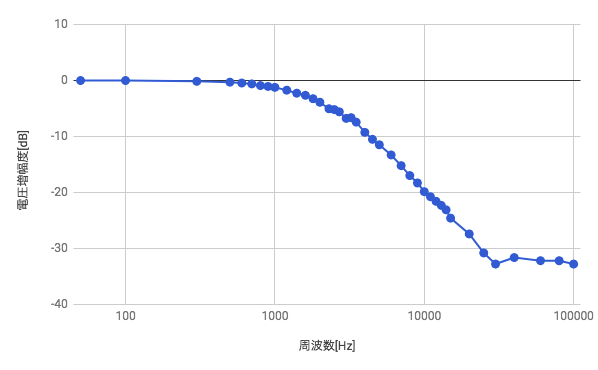
\includegraphics[width=8cm]{画像/ローパス対数.png}
		\caption{ローパスフィルタにおける周波数$f$と電圧増幅度$G$を示す片対数グラフ}
		\label{ローパス片対数}
	\end{center}
\end{figure}

\begin{figure}[H]
	\begin{center}
		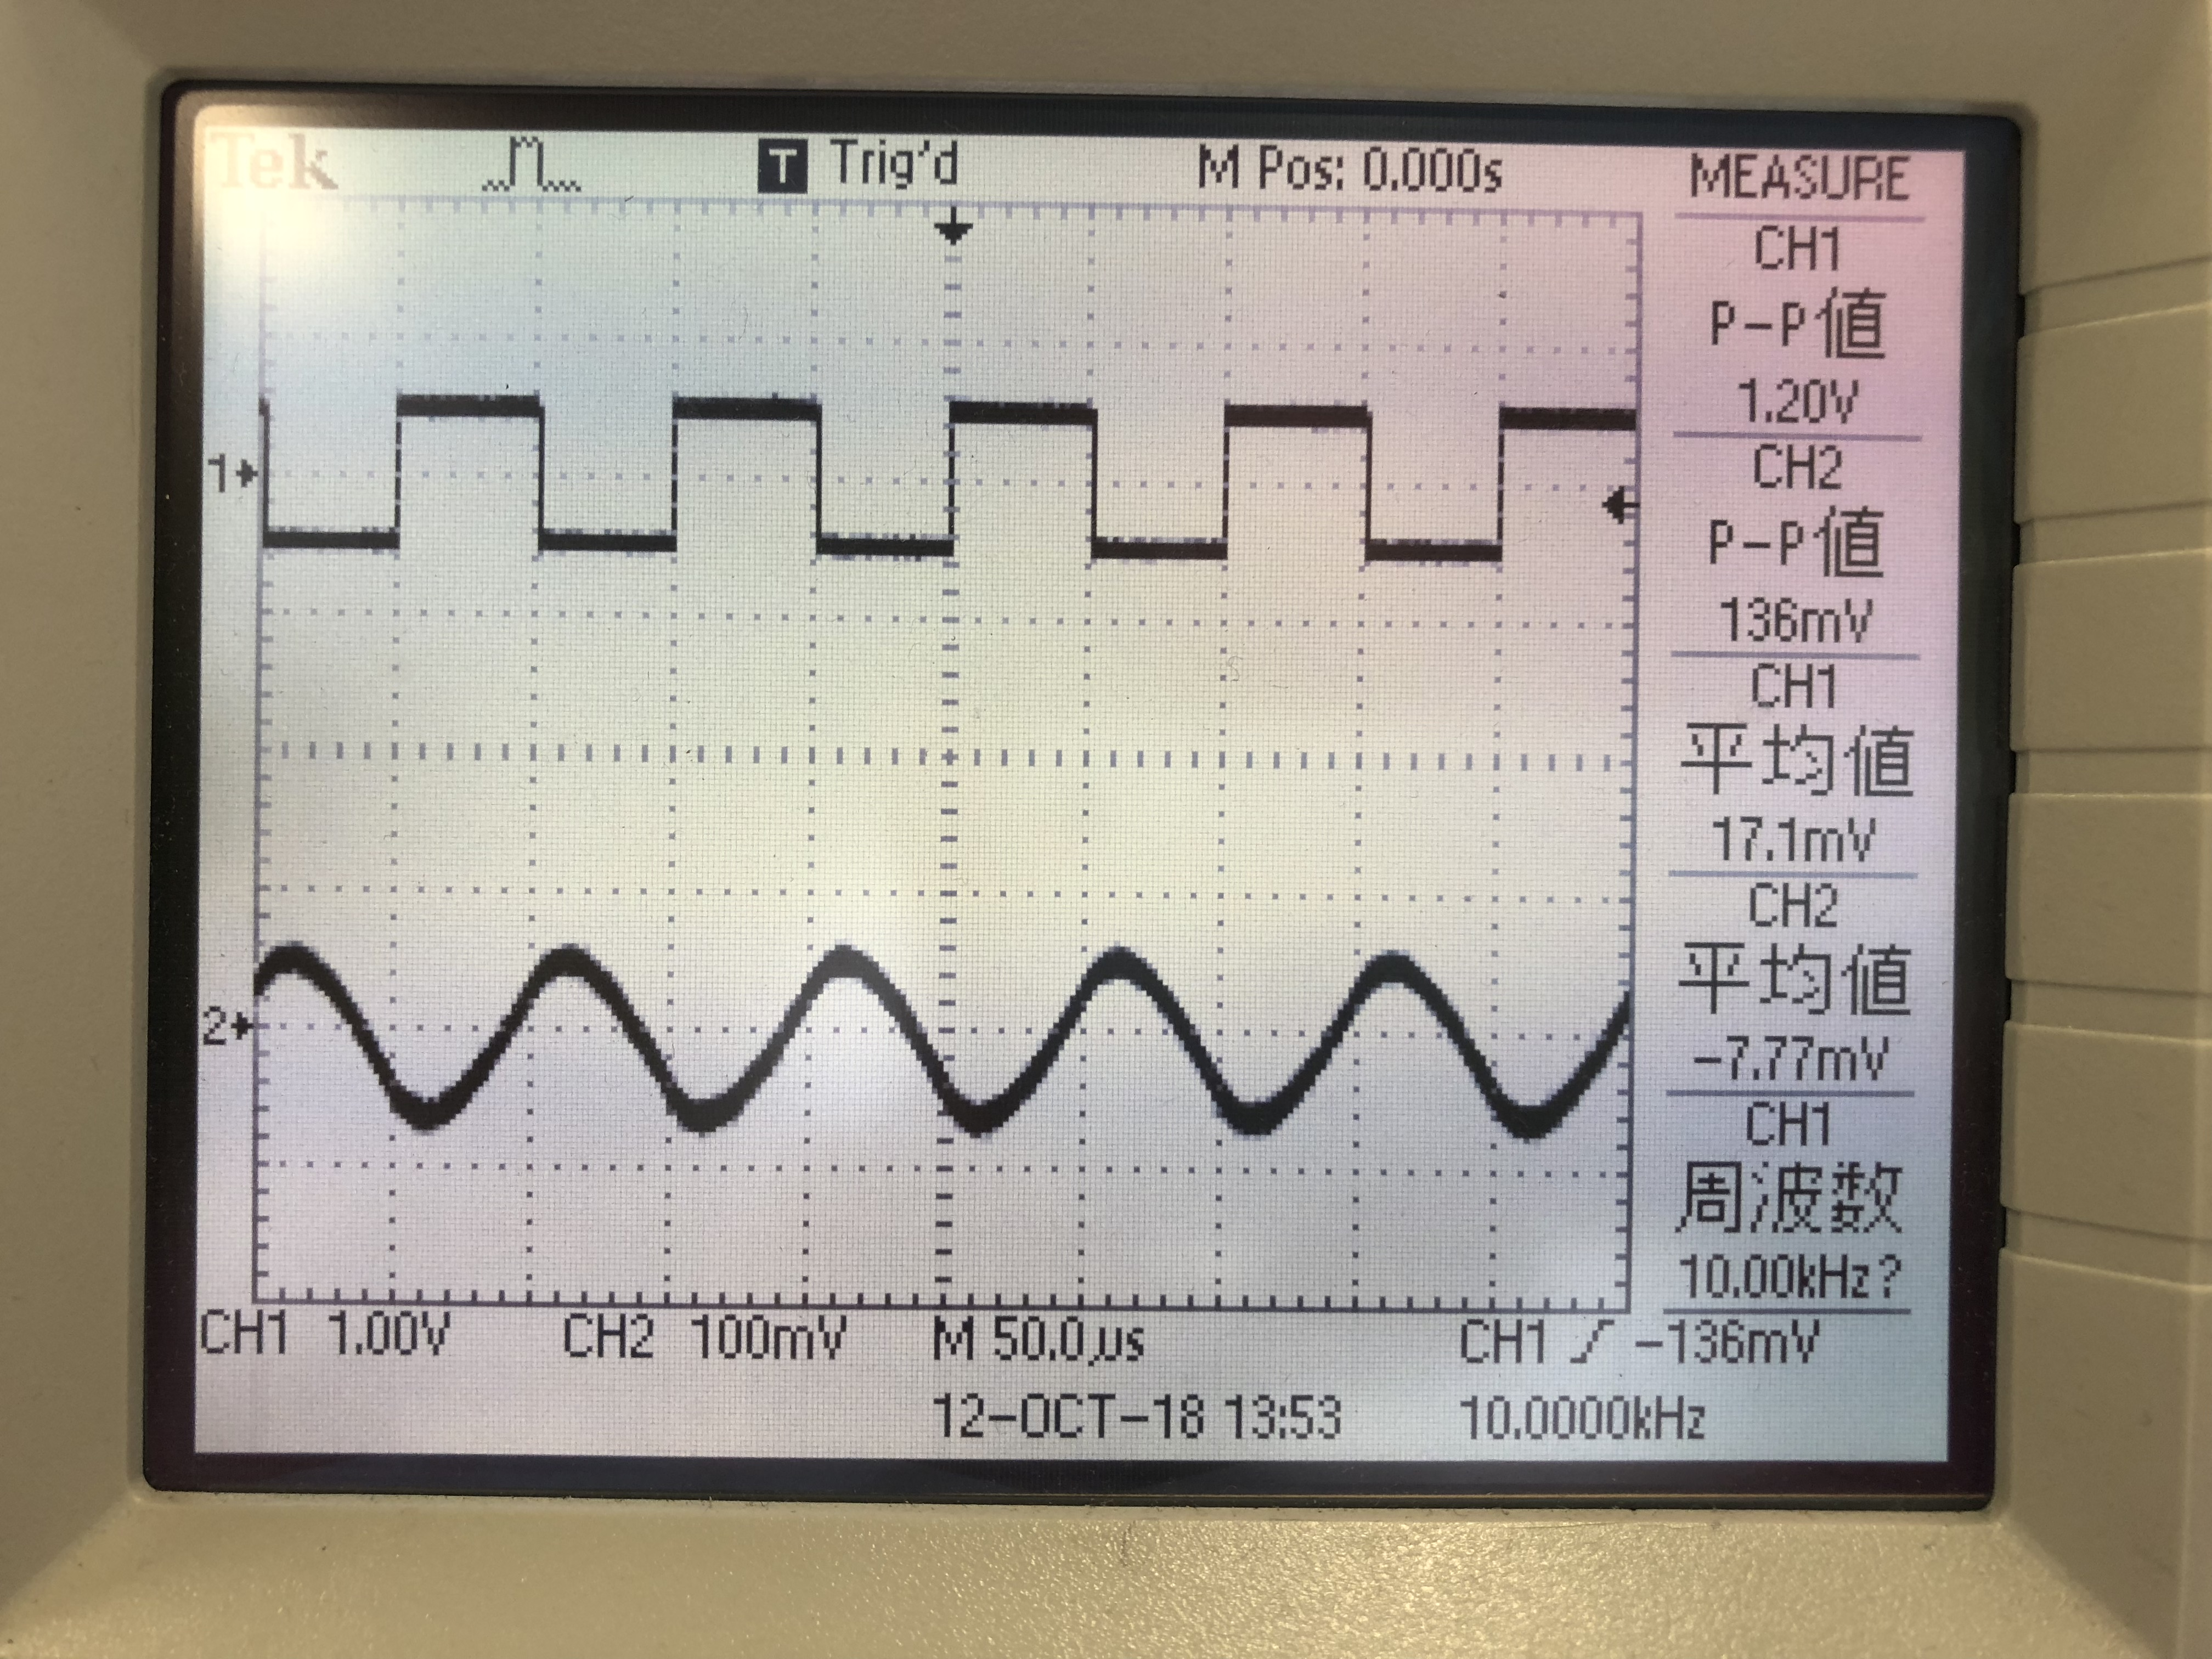
\includegraphics[width=8cm]{画像/ローパス方形波.jpg}
		\caption{10kHzの方形波を入力した時のローパスフィルタの出力波形}
		\label{ローパス方形波}
	\end{center}
\end{figure}

\subsection{ハイパスフィルタ回路}
回路に用いた抵抗とコンデンサの値と計算値を表\ref{ハイパス計算}に示す。
ハイパスフィルタの周波数特性は表\ref{ハイパス特性}と図\ref{ハイパス片対数}のようになった。
また、10kHzの方形波を入力した際の波形を図\ref{ハイパス方形波}に示した。
表\ref{ハイパス特性}と図\ref{ハイパス片対数}を見ると, 周波数をだんだんと下げていくと, 90000Hz付近から徐々に電圧増幅度の低下が始まり,
30000Hz付近からなだらかに低下していることがわかる. つまり, 高周波数帯では減衰させず、低周波数帯になるにつれ減衰が大きくなる回路であるとわかる.
図\ref{ハイパス方形波}の方形波では横線の部分が低周波数で縦線の部分が高周波数となっており、ハイパスフィルタを通すことで
高周波の部分だけが検出され、尖った波形になることがわかる.
\begin{table}[H]
	\caption{ハイパスフィルタ回路作成に用いた諸計算値}
	\label{ハイパス計算}
	\begin{center}
    \begin{tabular}[H]{|c|c|}\hline
      $R_1$[k$\Omega$] & 100 \\ \hline
      $R_2$[k$\Omega$] & 10\\ \hline
      $C_1$[$\mu$ F] & 0.0022\\ \hline
      $C_2$[$\mu$ F] & 0.0011 \\\hline
      $Q$ & 0.0149 \\ \hline
      $\omega_0$[rad/s] & $2.033\times10^4$ \\ \hline
      $f_0$[Hz] & 3235.8\\ \hline
    \end{tabular}
\end{center}
\end{table}

\begin{table}[H]
	\caption{ハイパスフィルタにおける周波数特性}
	\label{ハイパス特性}
	\begin{center}
    \begin{tabular}[H]{|c|c|c|c|}\hline
      Hz & 入力電圧$V_{in}$[$\mathrm{V_{p-p}}$] & 出力電圧$V_{out}$[$\mathrm{V_{p-p}}$] & 電圧増幅度$G$[dB]  \\ \hline
      100 & 1.18 & 0.0176 & -36.52738679 \\ \hline
      200 & 1.18 & 0.0184 & -36.14128369 \\ \hline
      300 & 1.18 & 0.0224 & -34.43267978 \\ \hline
      400 & 1.18 & 0.028 & -32.49447952 \\ \hline
      500 & 1.18 & 0.0352 & -30.50678688 \\ \hline
      600 & 1.18 & 0.0384 & -29.75101566 \\ \hline
      700 & 1.18 & 0.0448 & -28.41207987 \\ \hline
      800 & 1.18 & 0.0504 & -27.38902942 \\ \hline
      900 & 1.2 & 0.056 & -26.61986438 \\ \hline
      1000 & 1.18 & 0.0624 & -25.53394835 \\ \hline
      2000 & 1.18 & 0.124 & -19.56920644 \\ \hline
      3000 & 1.18 & 0.176 & -16.52738679 \\ \hline
      3235.3 & 1.2 & 0.188 & -16.10046794 \\ \hline
      4000 & 1.2 & 0.224 & -14.57866455 \\ \hline
      5000 & 1.2 & 0.288 & -12.39577517 \\ \hline
      6000 & 1.2 & 0.336 & -11.05683937 \\ \hline
      7000 & 1.2 & 0.376 & -10.07986802 \\ \hline
      8000 & 1.2 & 0.416 & -9.201758308 \\ \hline
      9000 & 1.2 & 0.464 & -8.25326531 \\ \hline
      10000 & 1.22 & 0.512 & -7.541797394 \\ \hline
      20000 & 1.2 & 0.82 & -3.307347873 \\ \hline
      30000 & 1.18 & 0.94 & -1.975083074 \\ \hline
      40000 & 1.18 & 1.02 & -1.265636711 \\ \hline
      50000 & 1.2 & 1.06 & -1.077507616 \\ \hline
      60000 & 1.2 & 1.1 & -0.7557712178 \\ \hline
      70000 & 1.2 & 1.1 & -0.7557712178 \\ \hline
      80000 & 1.2 & 1.12 & -0.5992644675 \\ \hline
      90000 & 1.22 & 1.18 & -0.2895564674 \\ \hline
      100000 & 1.22 & 1.18 & -0.2895564674 \\ \hline
      300000 & 1.22 & 1.22 & 0 \\ \hline
      500000 & 1.24 & 1.22 & -0.1412370897 \\ \hline
    \end{tabular}
\end{center}
\end{table}

\begin{figure}[H]
	\begin{center}
		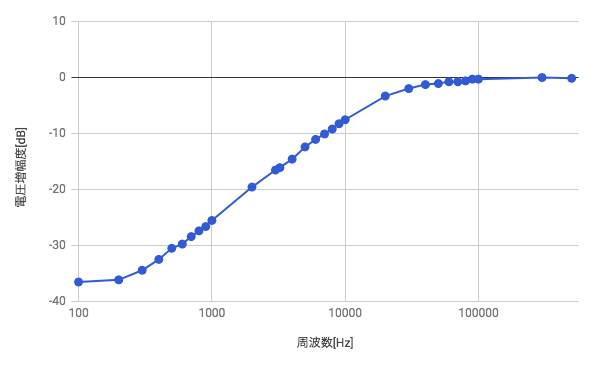
\includegraphics[width=8cm]{画像/ハイパス方対数.png}
		\caption{ハイパスフィルタにおける周波数$f$と電圧増幅度$G$を示す片対数グラフ}
		\label{ハイパス片対数}
	\end{center}
\end{figure}

\begin{figure}[H]
	\begin{center}
		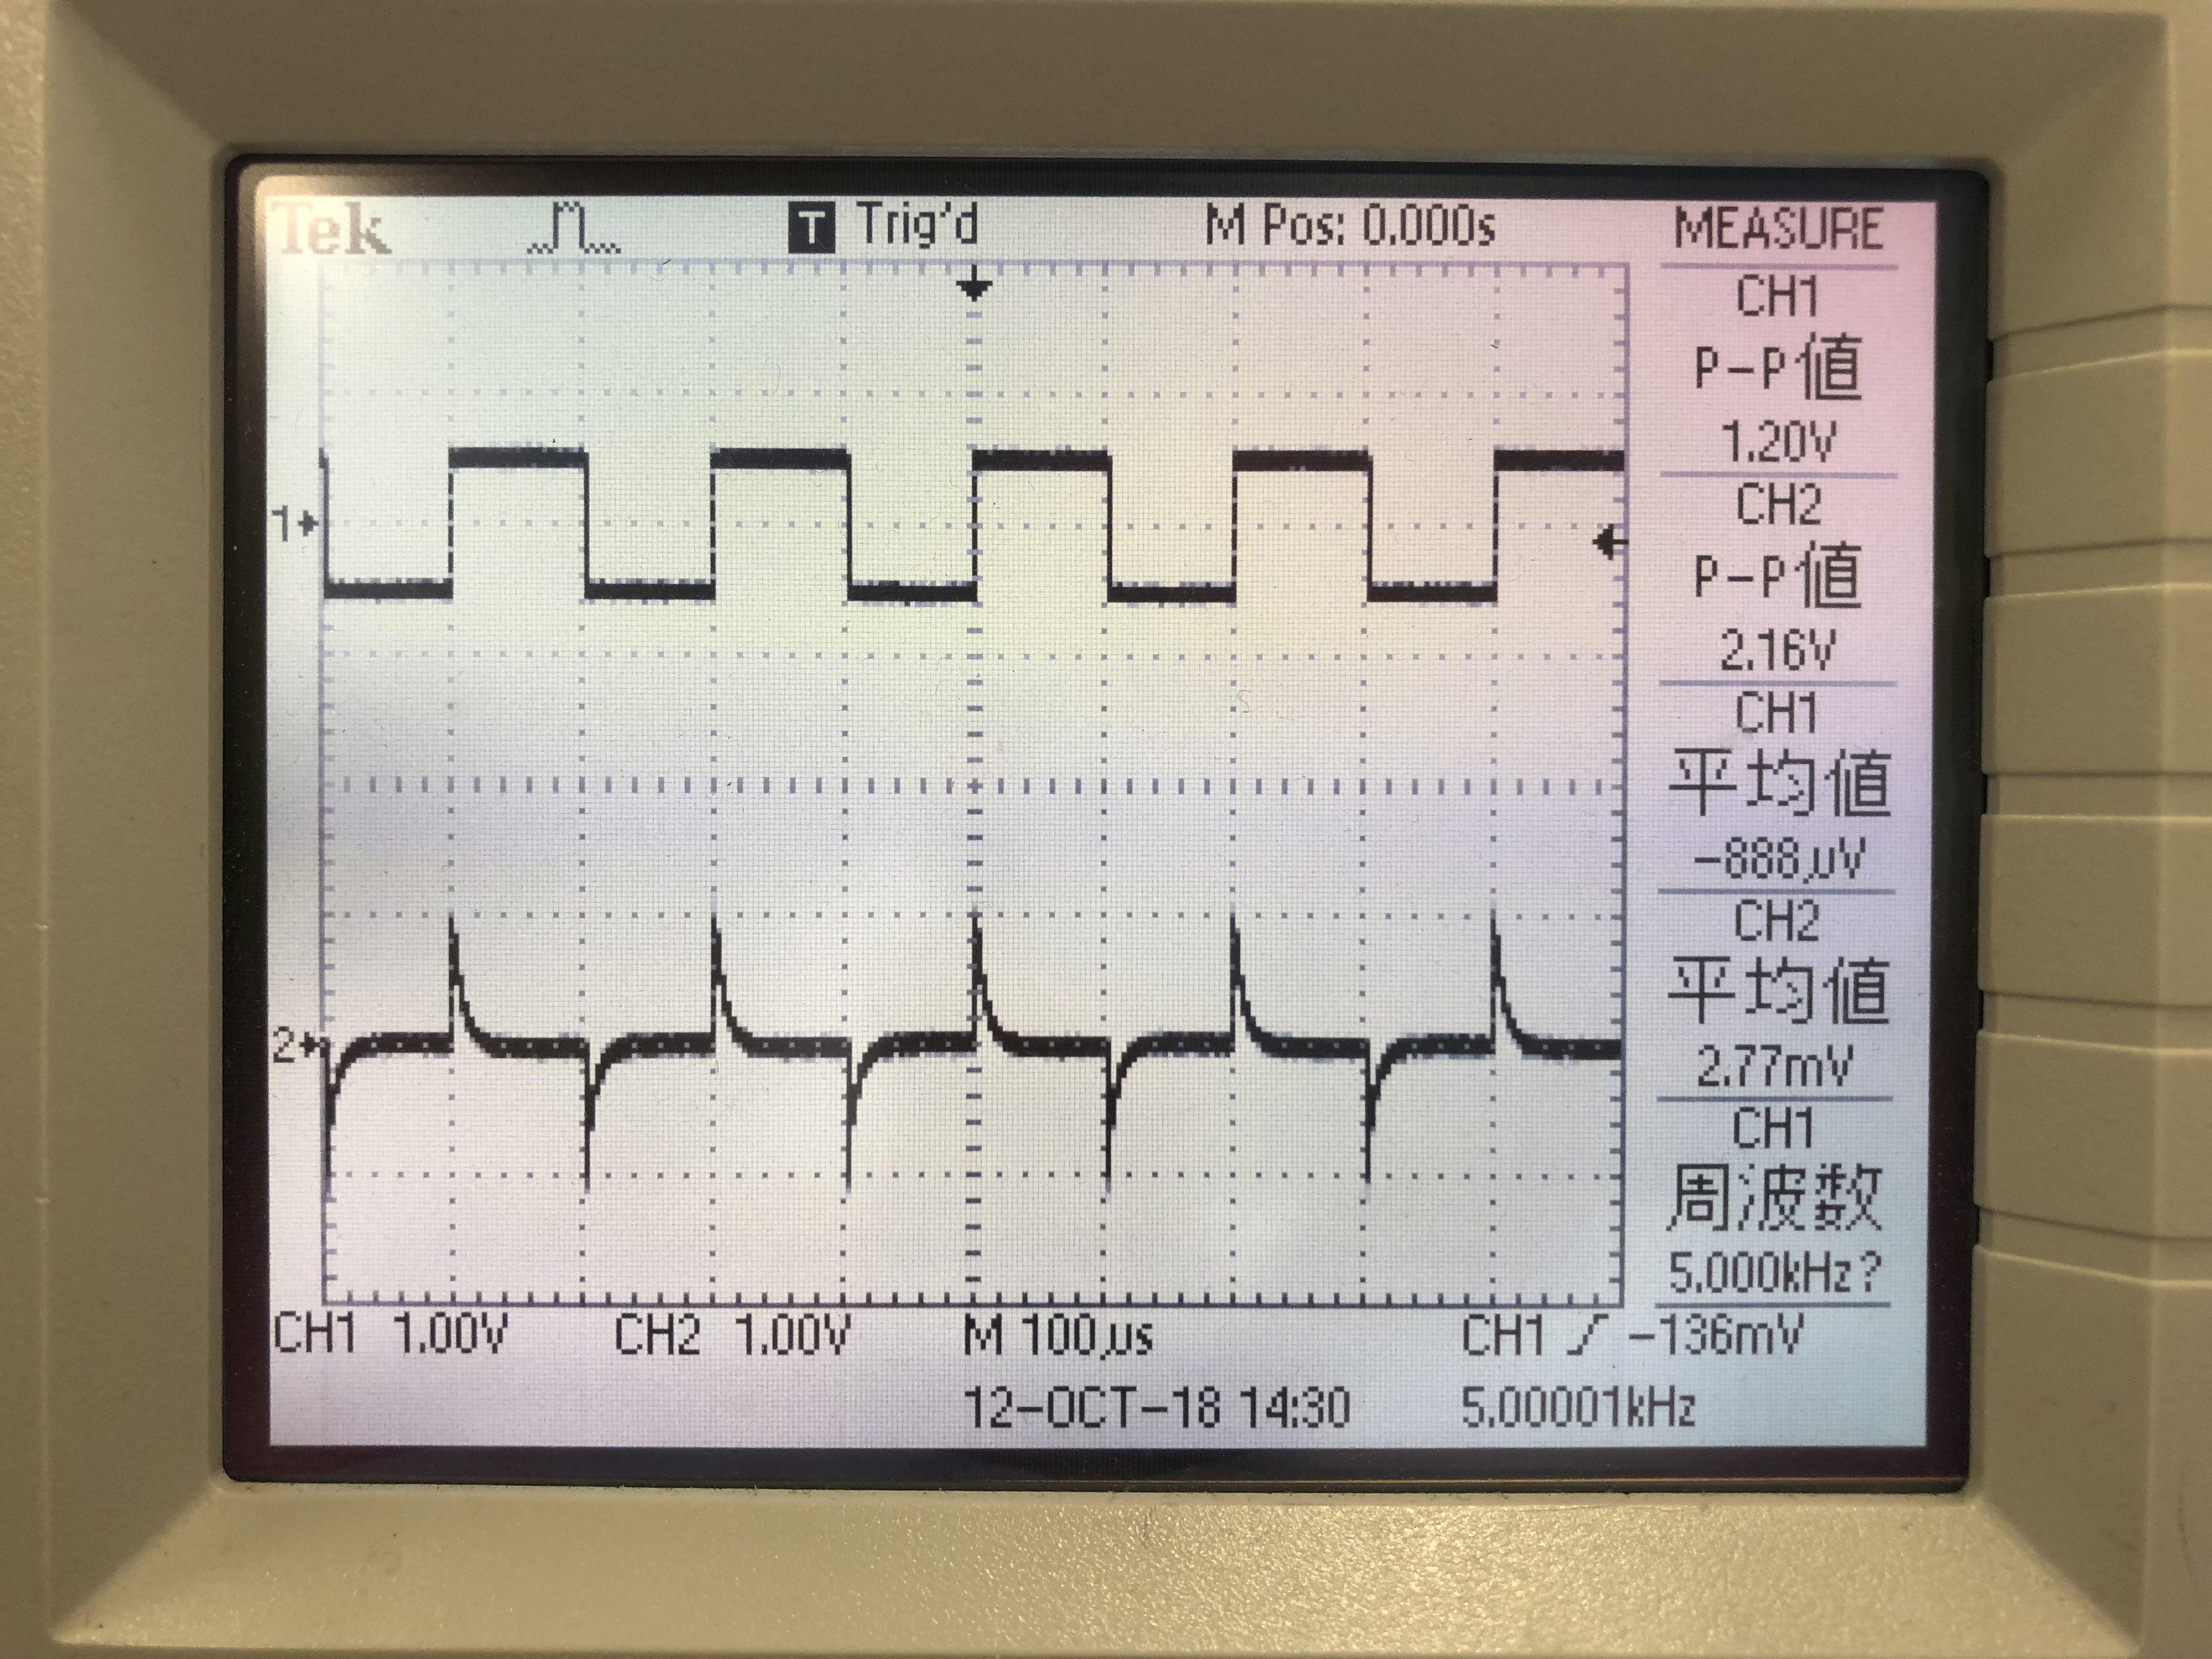
\includegraphics[width=8cm]{画像/ハイパス方形波.jpg}
		\caption{10kHzの方形波を入力した時のハイパスフィルタの出力波形}
		\label{ハイパス方形波}
	\end{center}
\end{figure}

\subsection{微分回路}
微分器として安全な下限の周波数$f_s$は、$f_s=1.592 \times 10^3$Hzとなった。
$f_s$を基準として3通りに周波数を変更した際の波形は以下のグラフのようになった(図21($f<f_s$),図22($f=f_s$), 図23($f>f_s$))。

$f$が安定上限より小さい時(図21)では、方形波の傾きに正確に表している。
$f$が安定上限と等しい時(図22)では、傾きを表すとがりの根元が半周期分まで到達している。
$f$が安定上限より大きい時(図23)では、微分器としての機能は完全に失い、波形を反転させている。

\begin{figure}[H]
	\begin{center}
		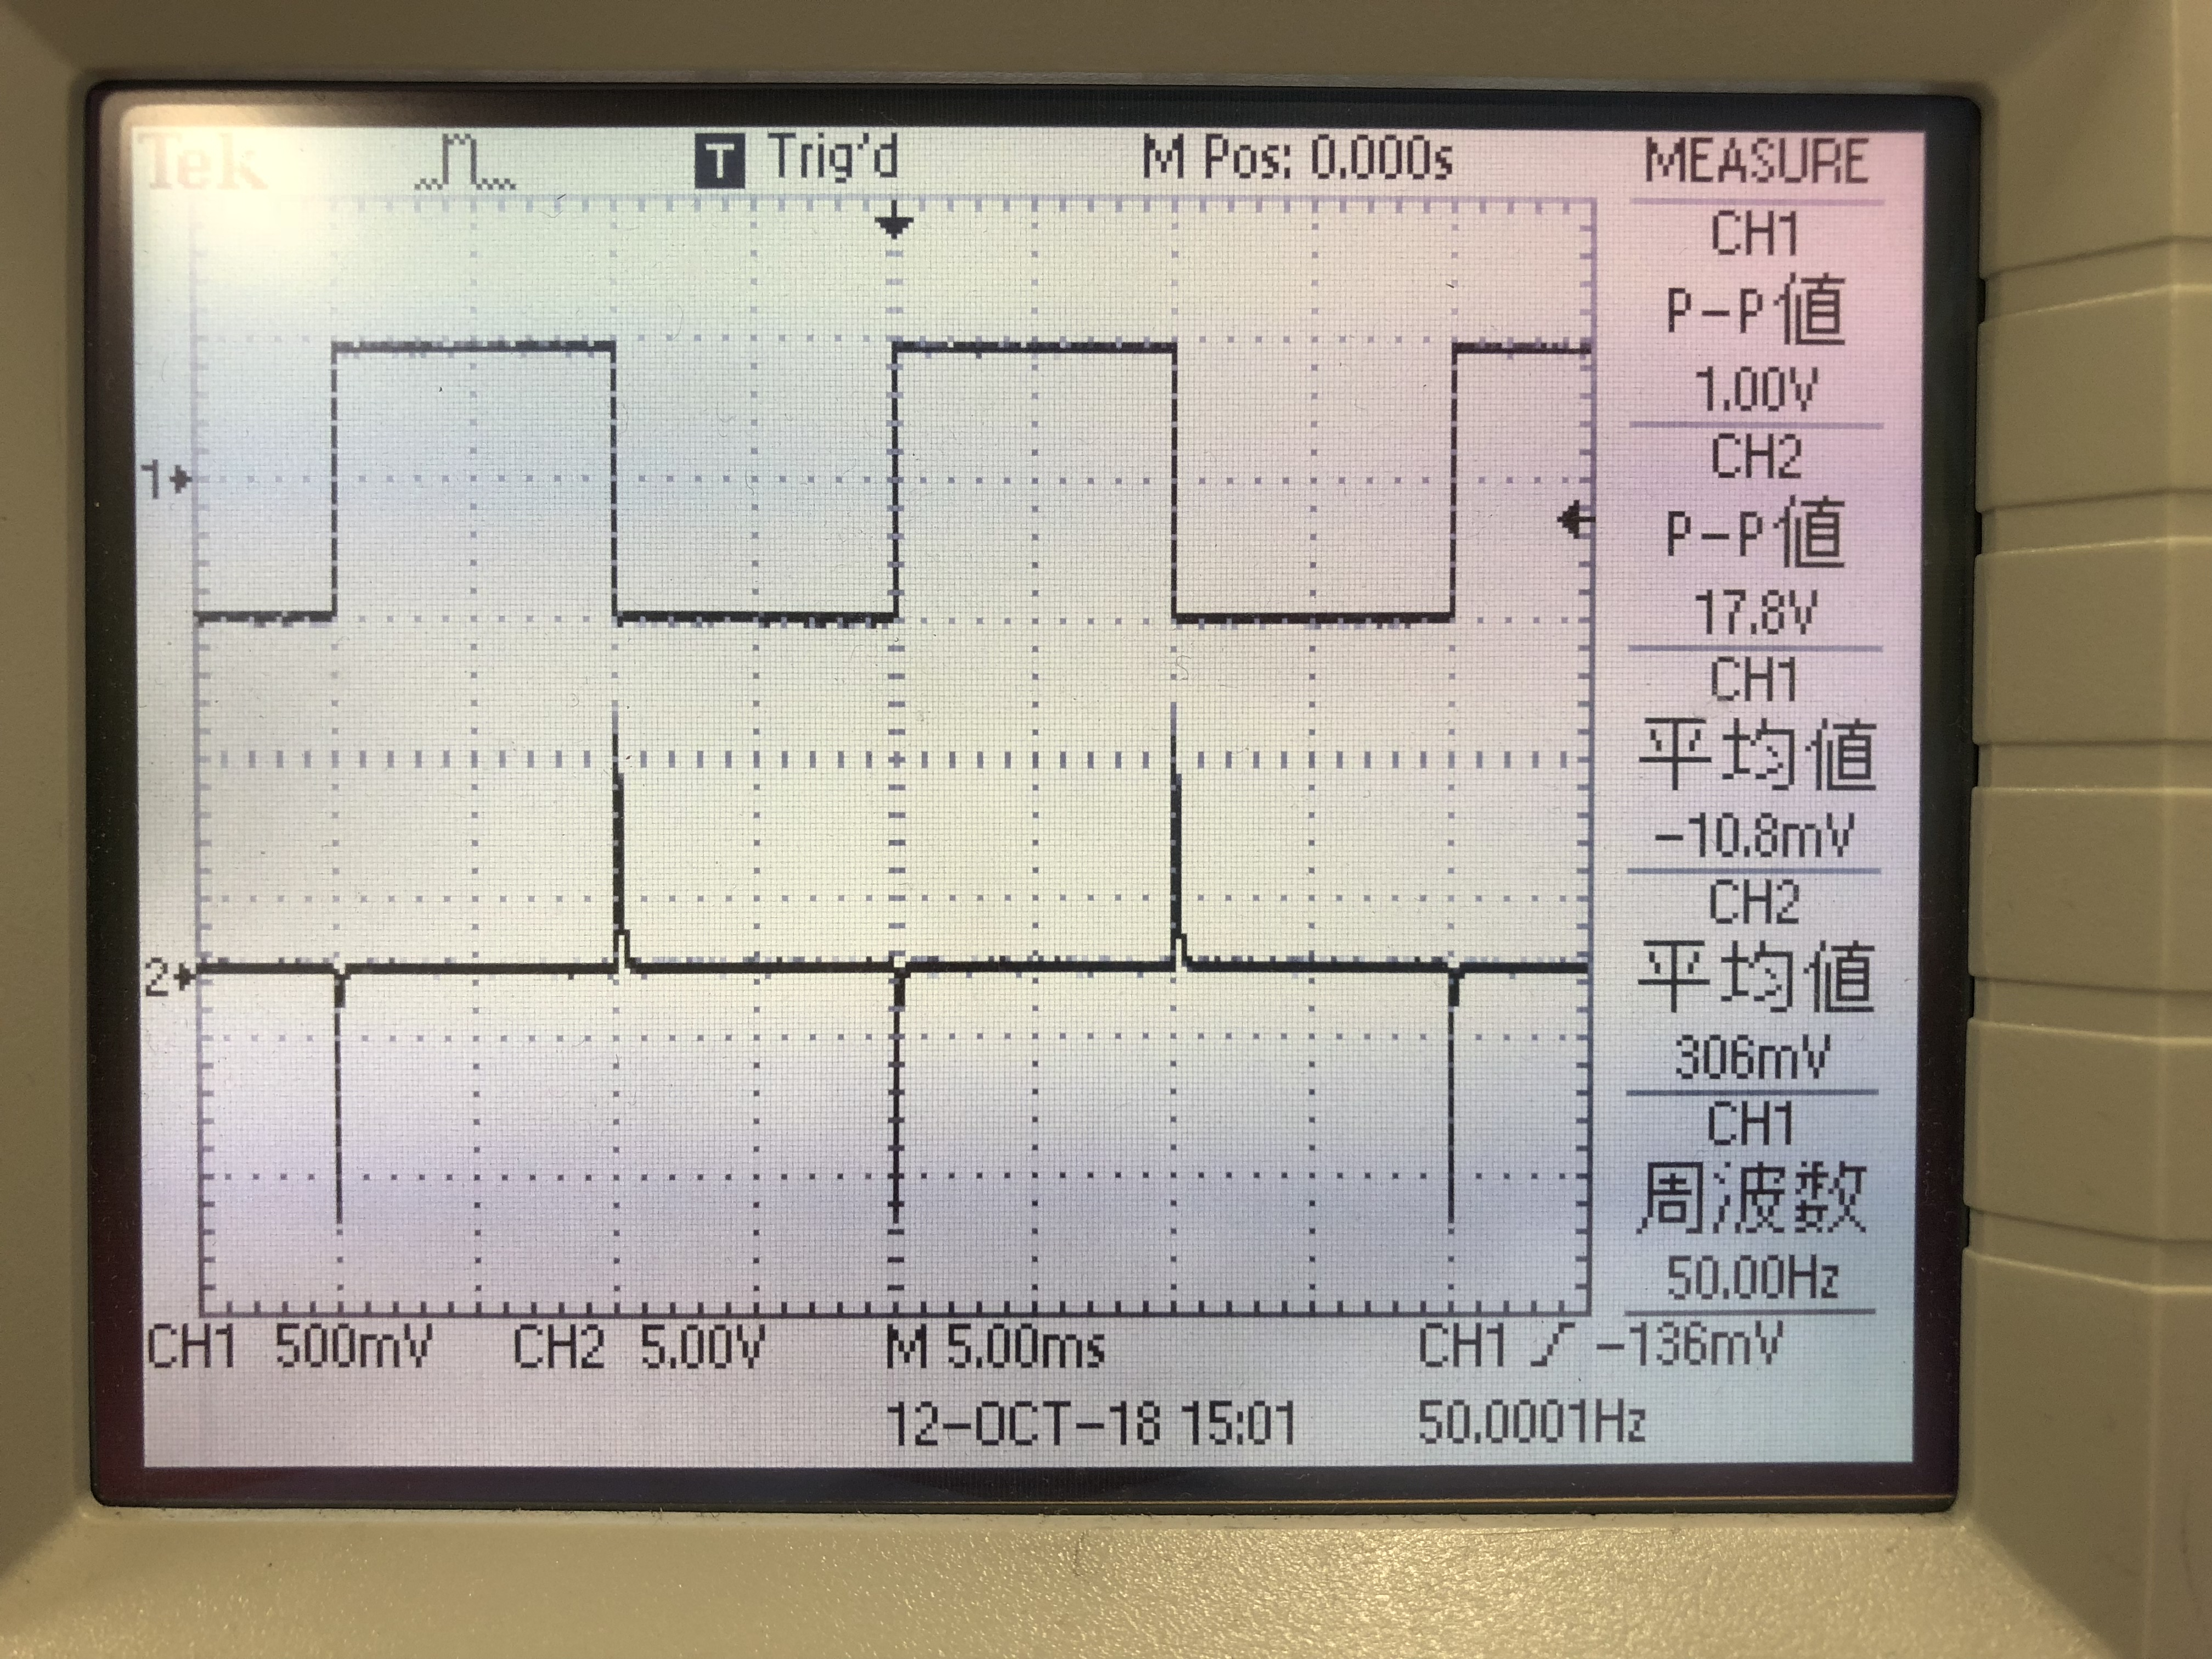
\includegraphics[width=8cm]{画像/f<fs.jpg}
		\caption{微分回路の出力波形($f<f_s$の時)}
	\end{center}
\end{figure}

\begin{figure}[H]
	\begin{center}
		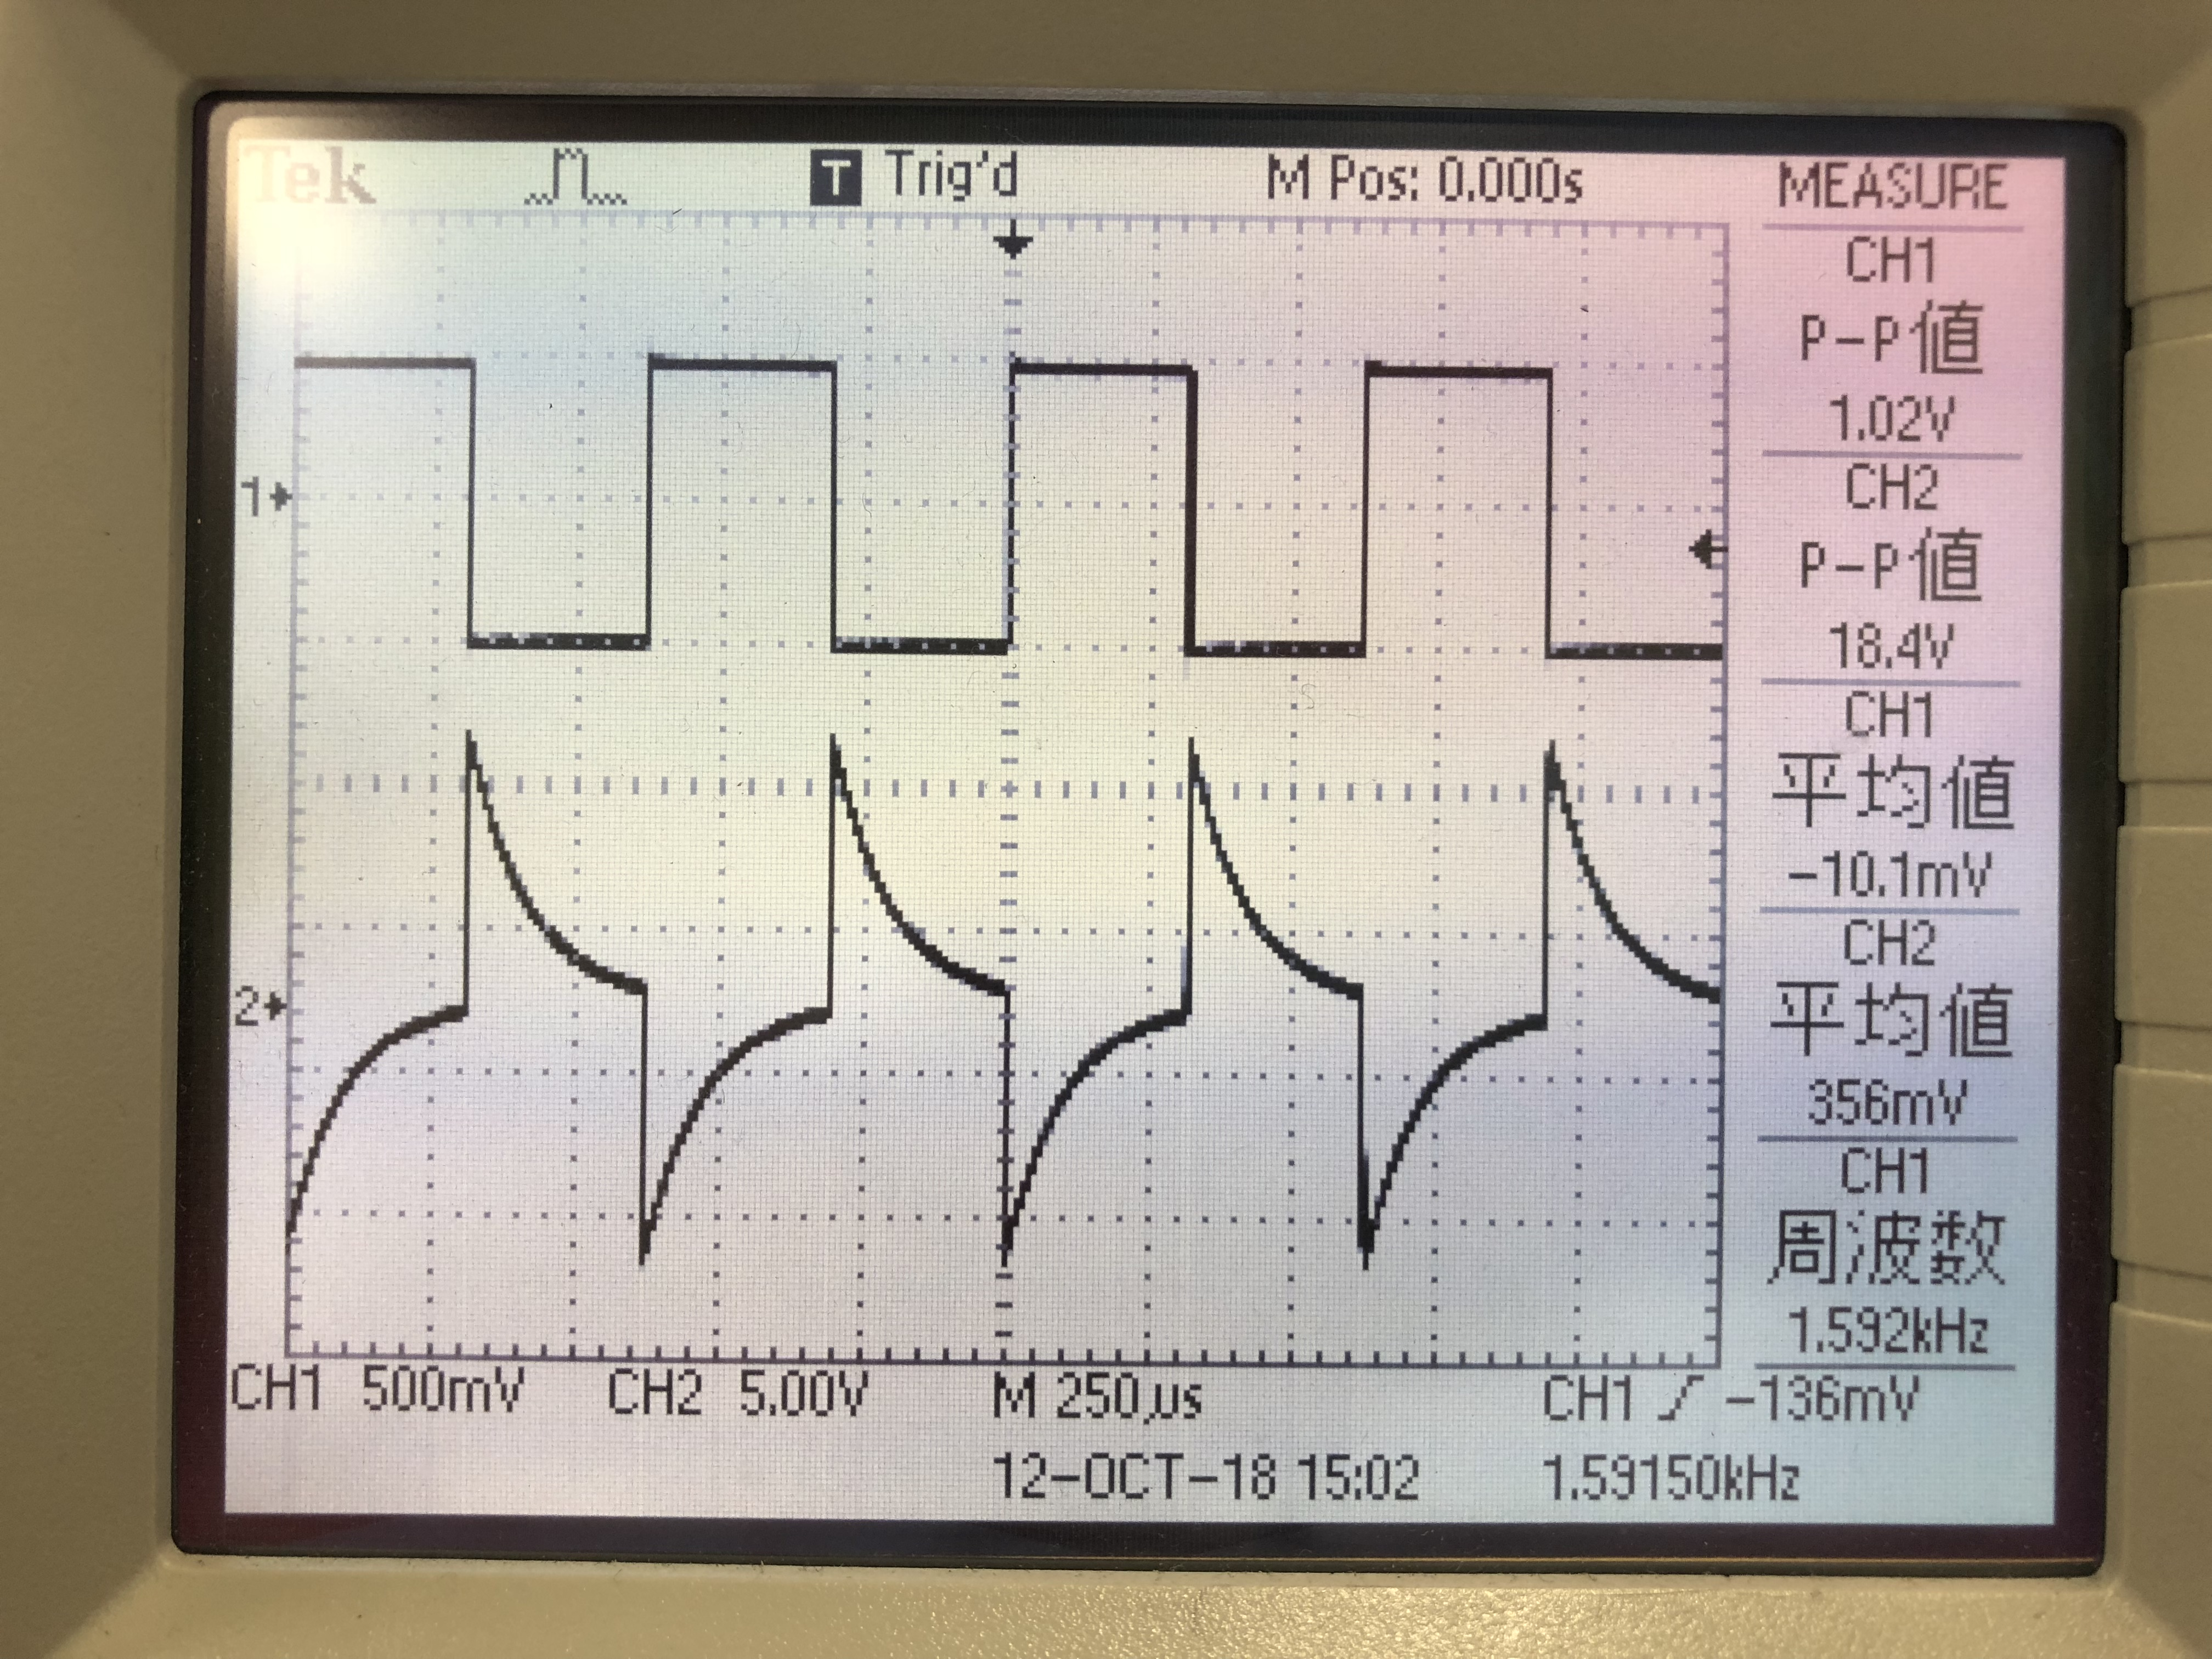
\includegraphics[width=8cm]{画像/f=fs.jpg}
		\caption{微分回路の出力波形($f=f_s$の時)}
	\end{center}
\end{figure}

\begin{figure}[H]
	\begin{center}
		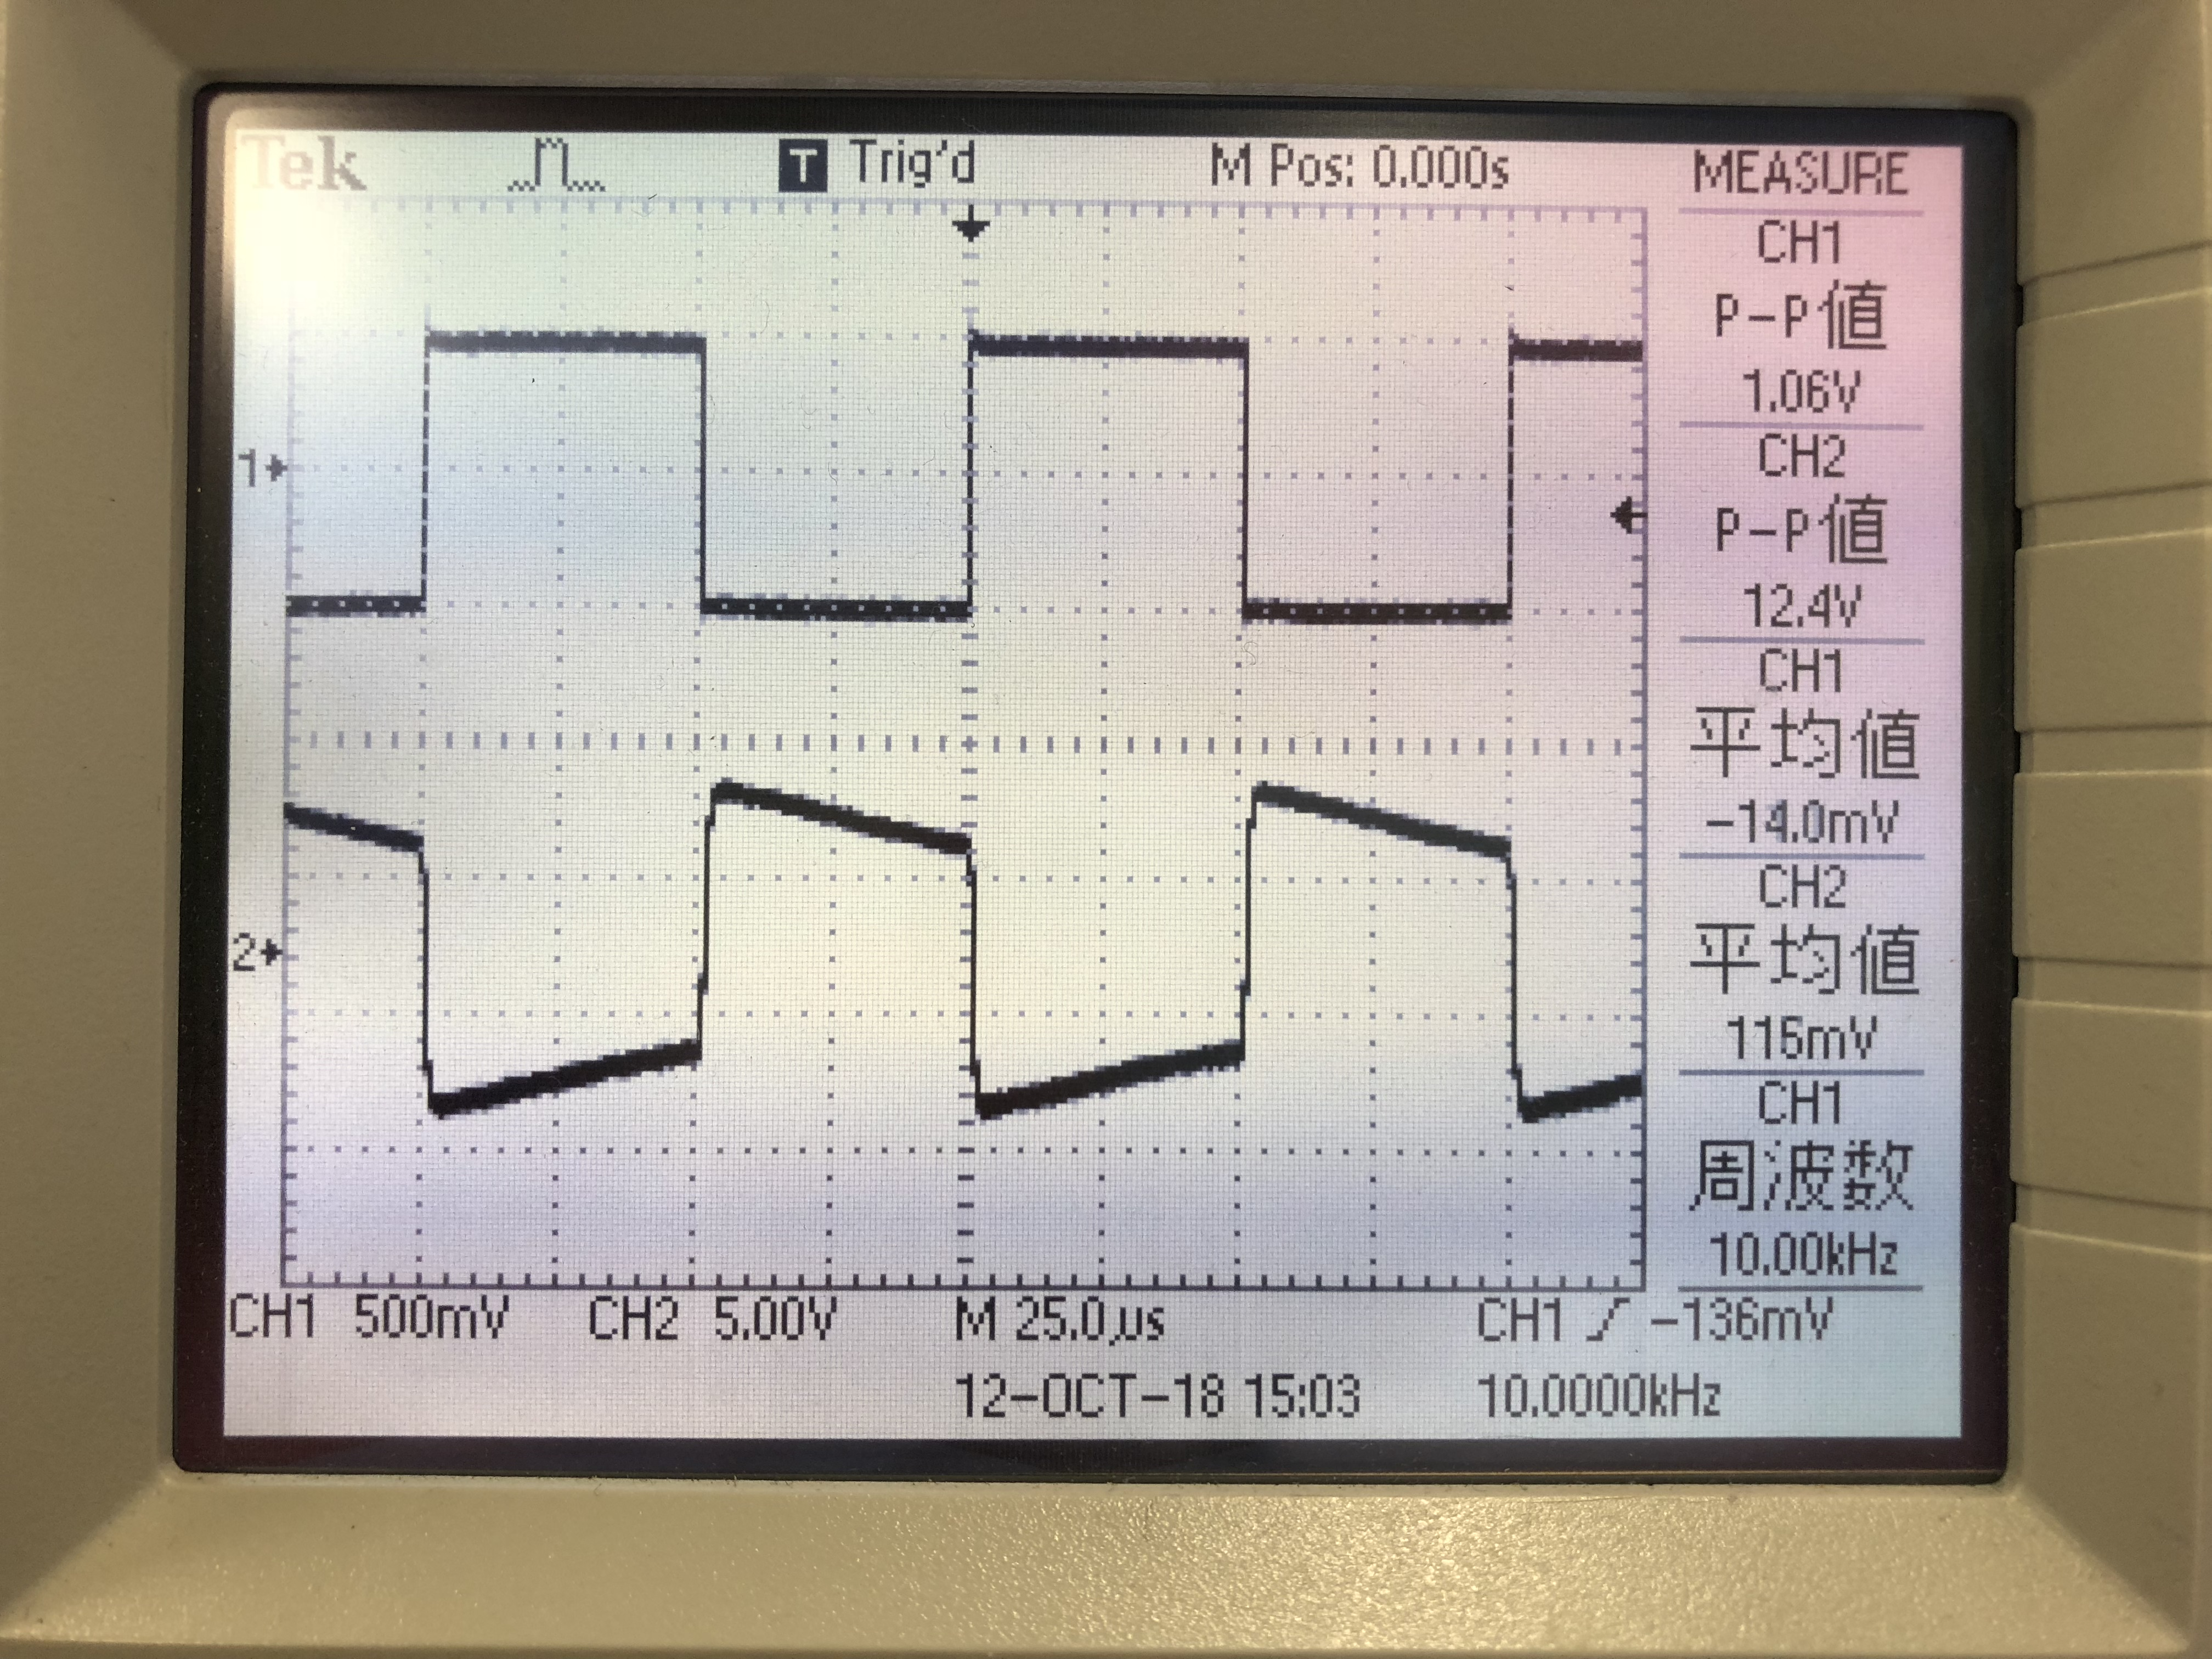
\includegraphics[width=8cm]{画像/f>fs.jpg}
		\caption{微分回路の出力波形($f>f_s$の時)}
	\end{center}
\end{figure}

\subsection{積分回路}
微分器として安全な下限の周波数$f_p$は、$f_p=723.43$Hzとなった。
$f_p$を基準として3通りに周波数を変更した際の波形は以下のグラフのようになった(図24($f>f_p$)),図25($f=f_p$),図26($f<f_p$))。
$f$が安定下限より大きい時(図24)では、方形波を積分した三角波になっており、積分器として機能していることがわかる。
$f$が安定下限と等しい時(図25)では、三角波が大きくゆがんでしまっている。
$f$が安定下限より小さい時(図26)では、完全に反転しており、積分器としての機能は失われてしまっている。
\begin{figure}[H]
	\begin{center}
		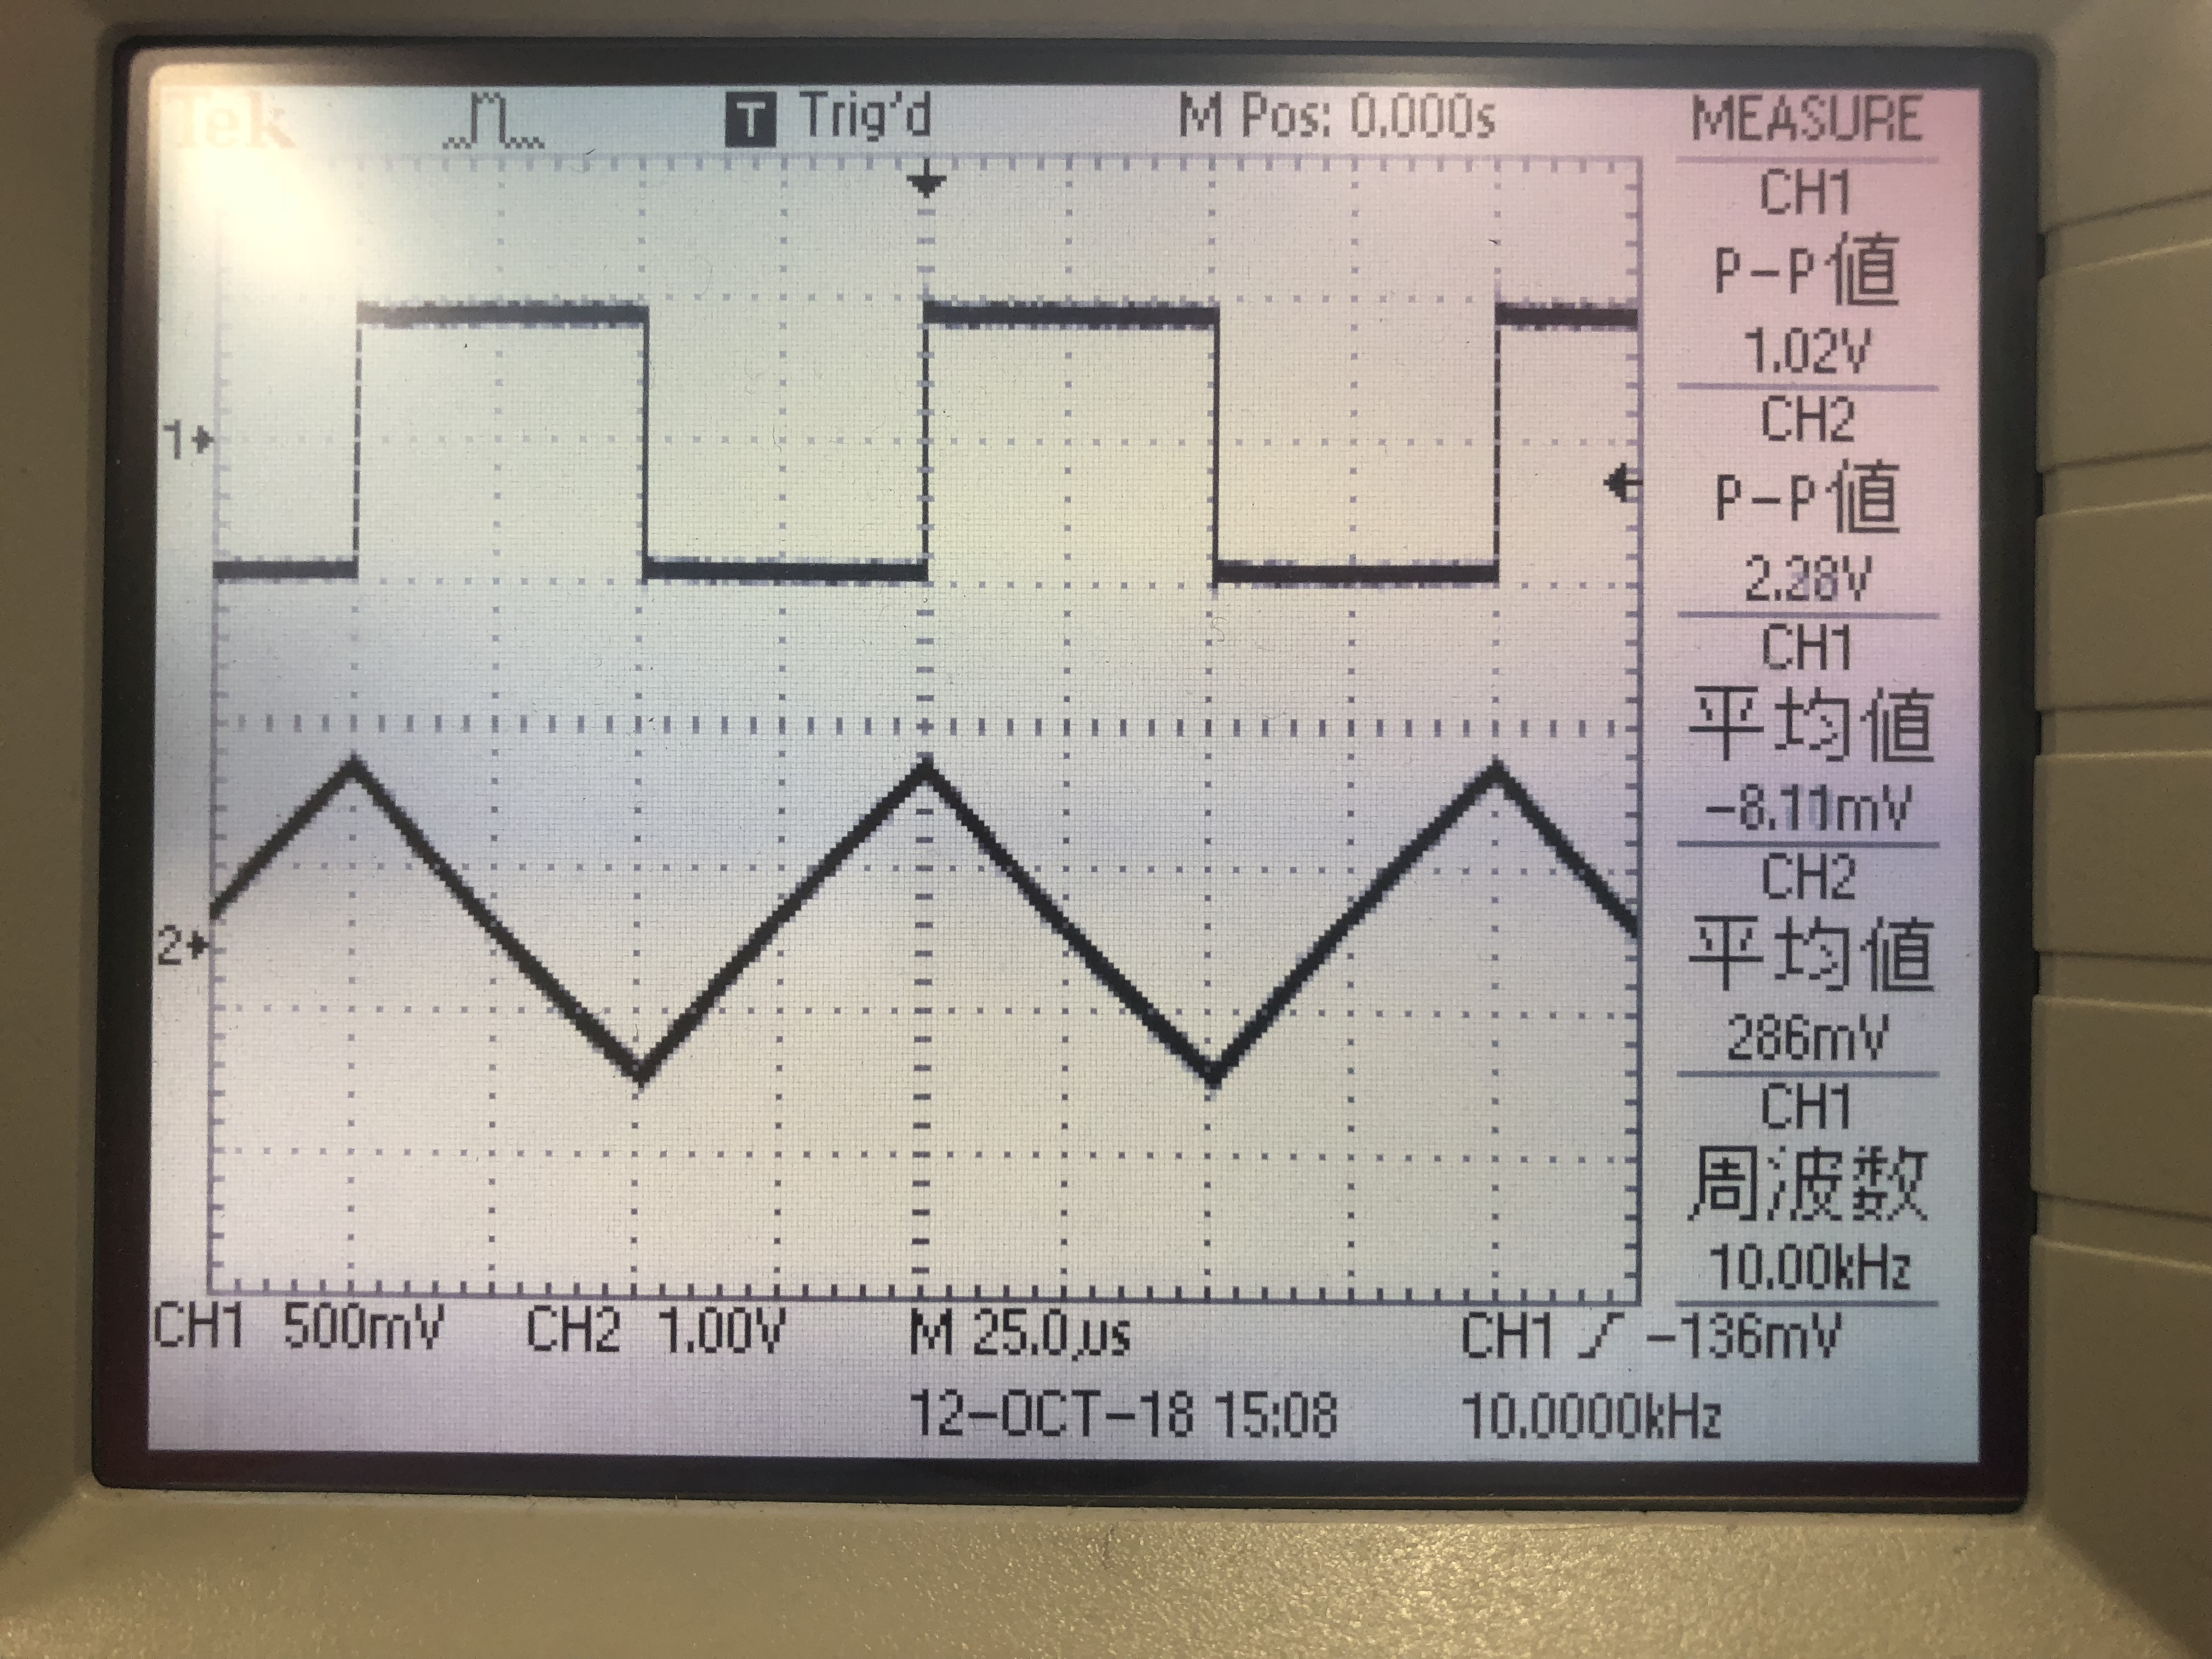
\includegraphics[width=8cm]{画像/f>fp.jpg}
		\caption{積分回路の出力波形($f>f_p$の時)}
	\end{center}
\end{figure}

\begin{figure}[H]
	\begin{center}
		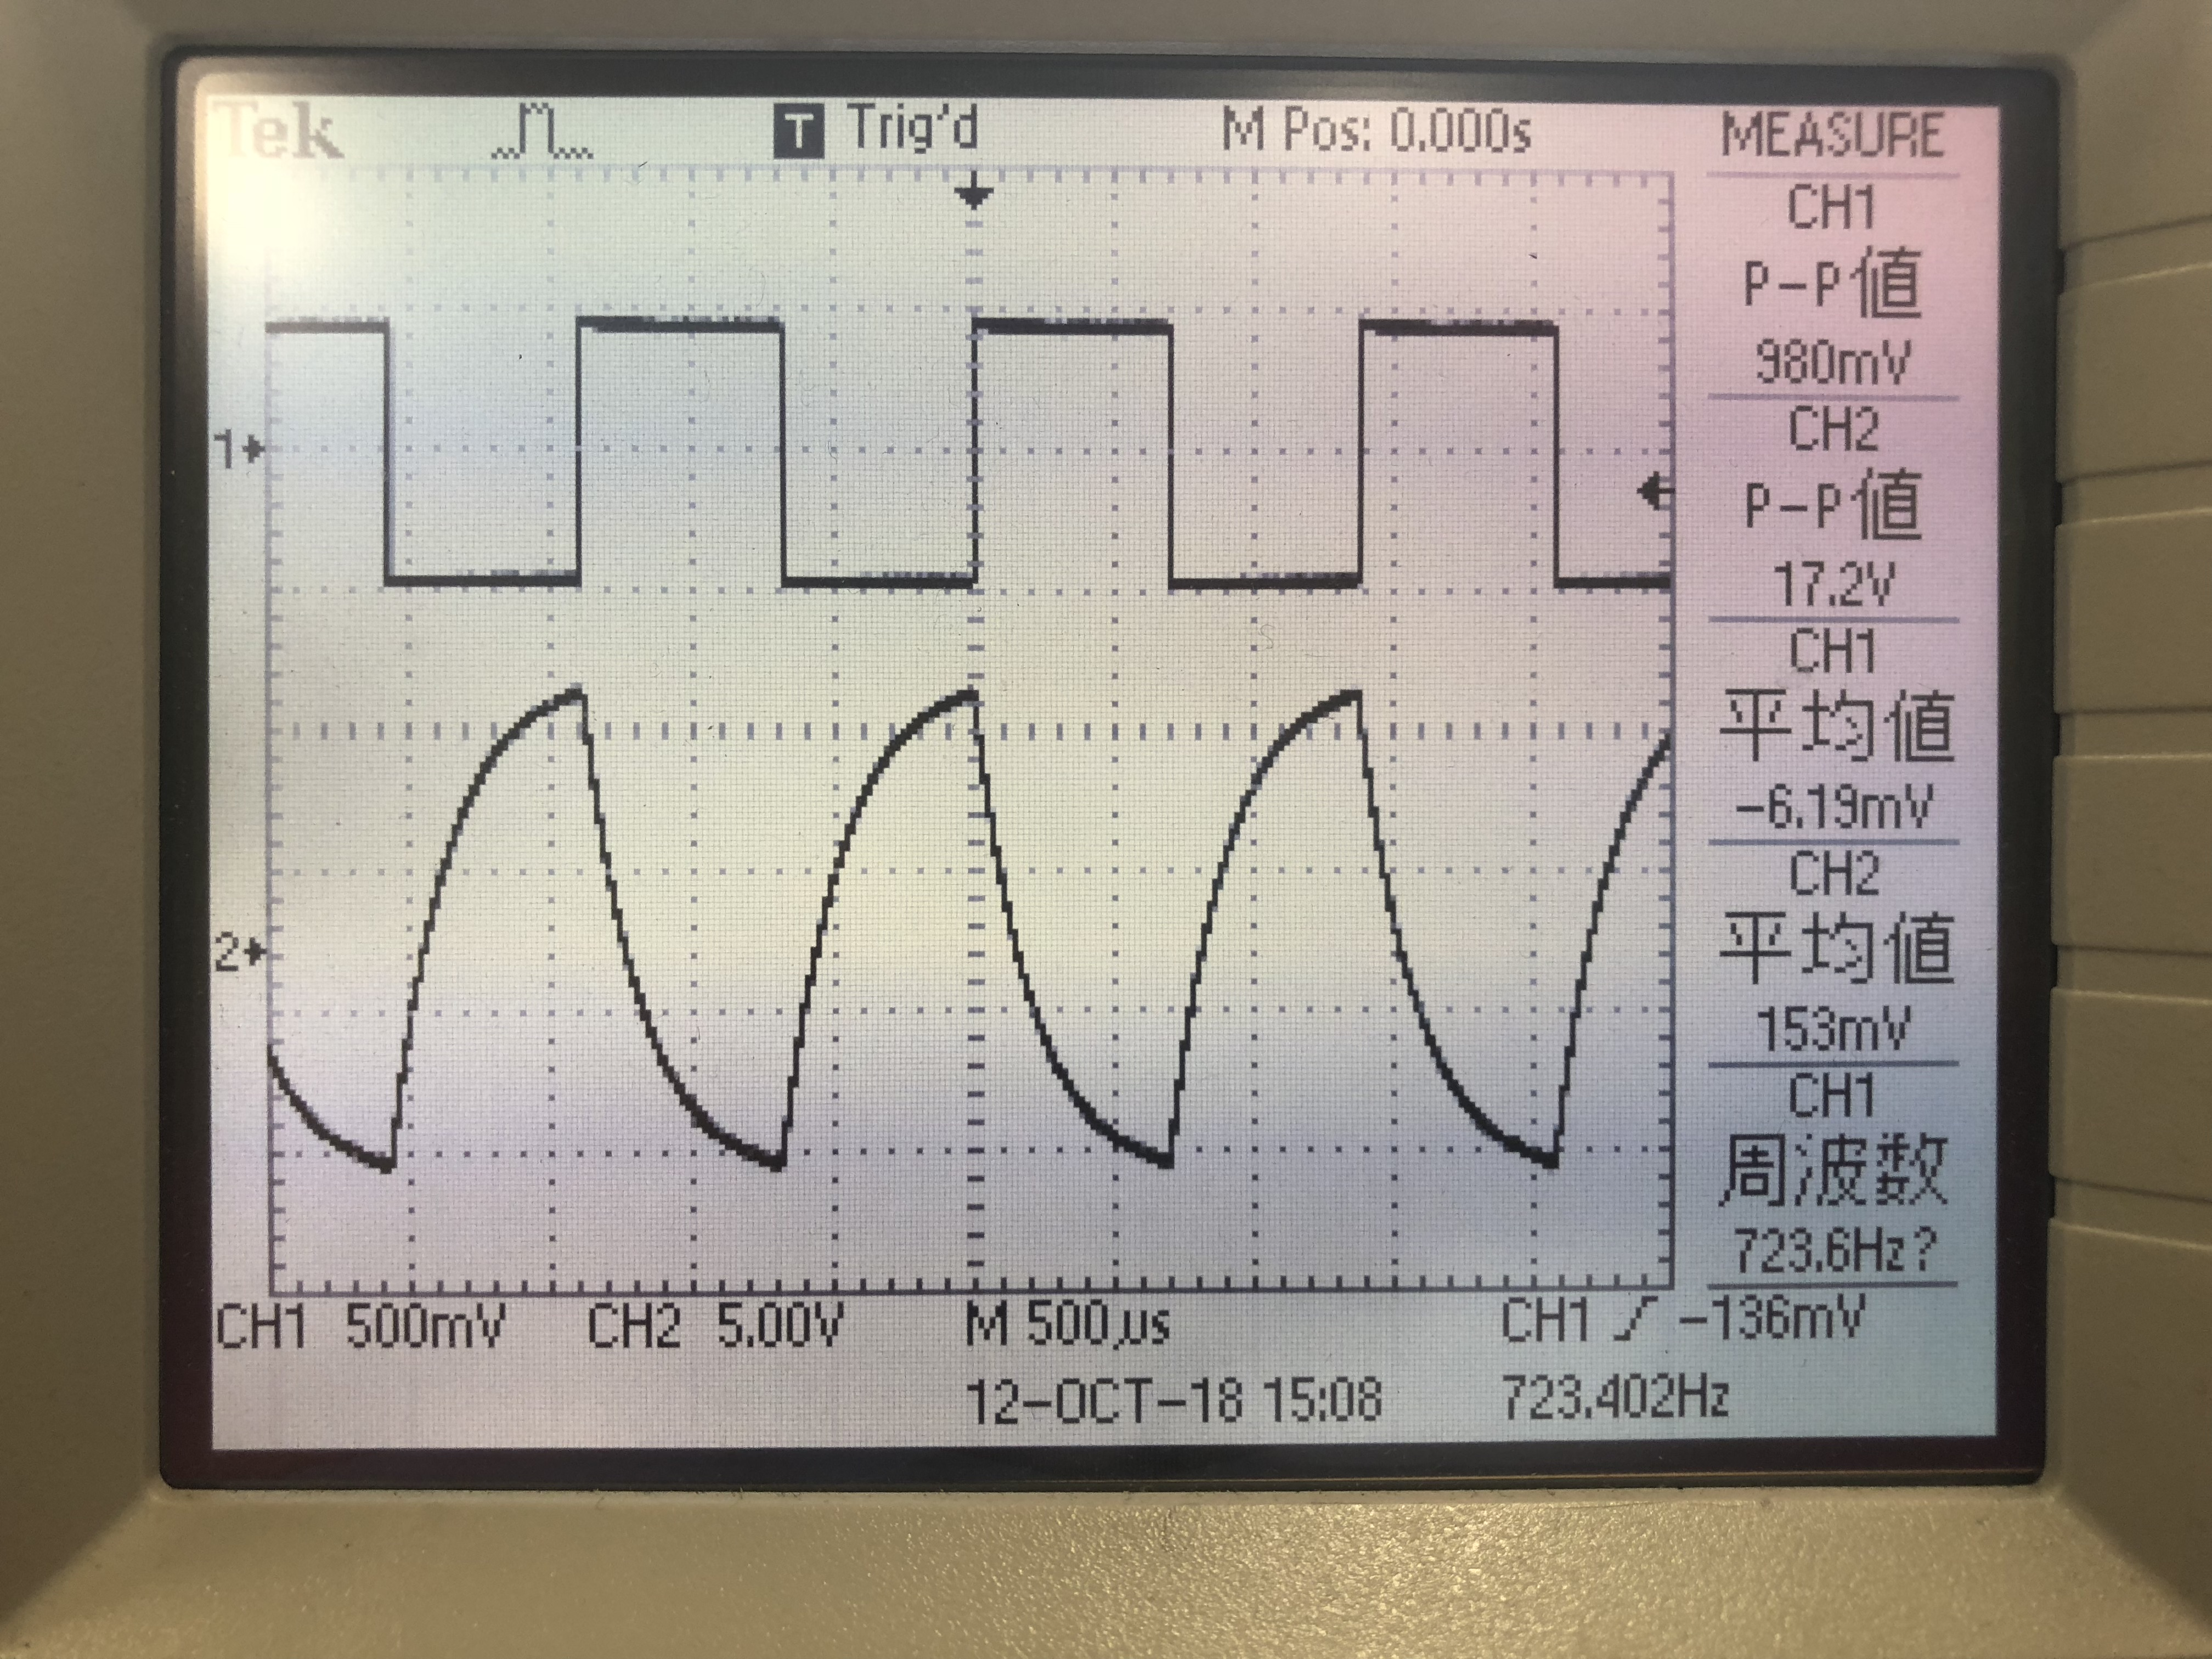
\includegraphics[width=8cm]{画像/f=fp.jpg}
		\caption{積分回路の出力波形($f=f_p$の時)}
	\end{center}
\end{figure}

\begin{figure}[H]
	\begin{center}
		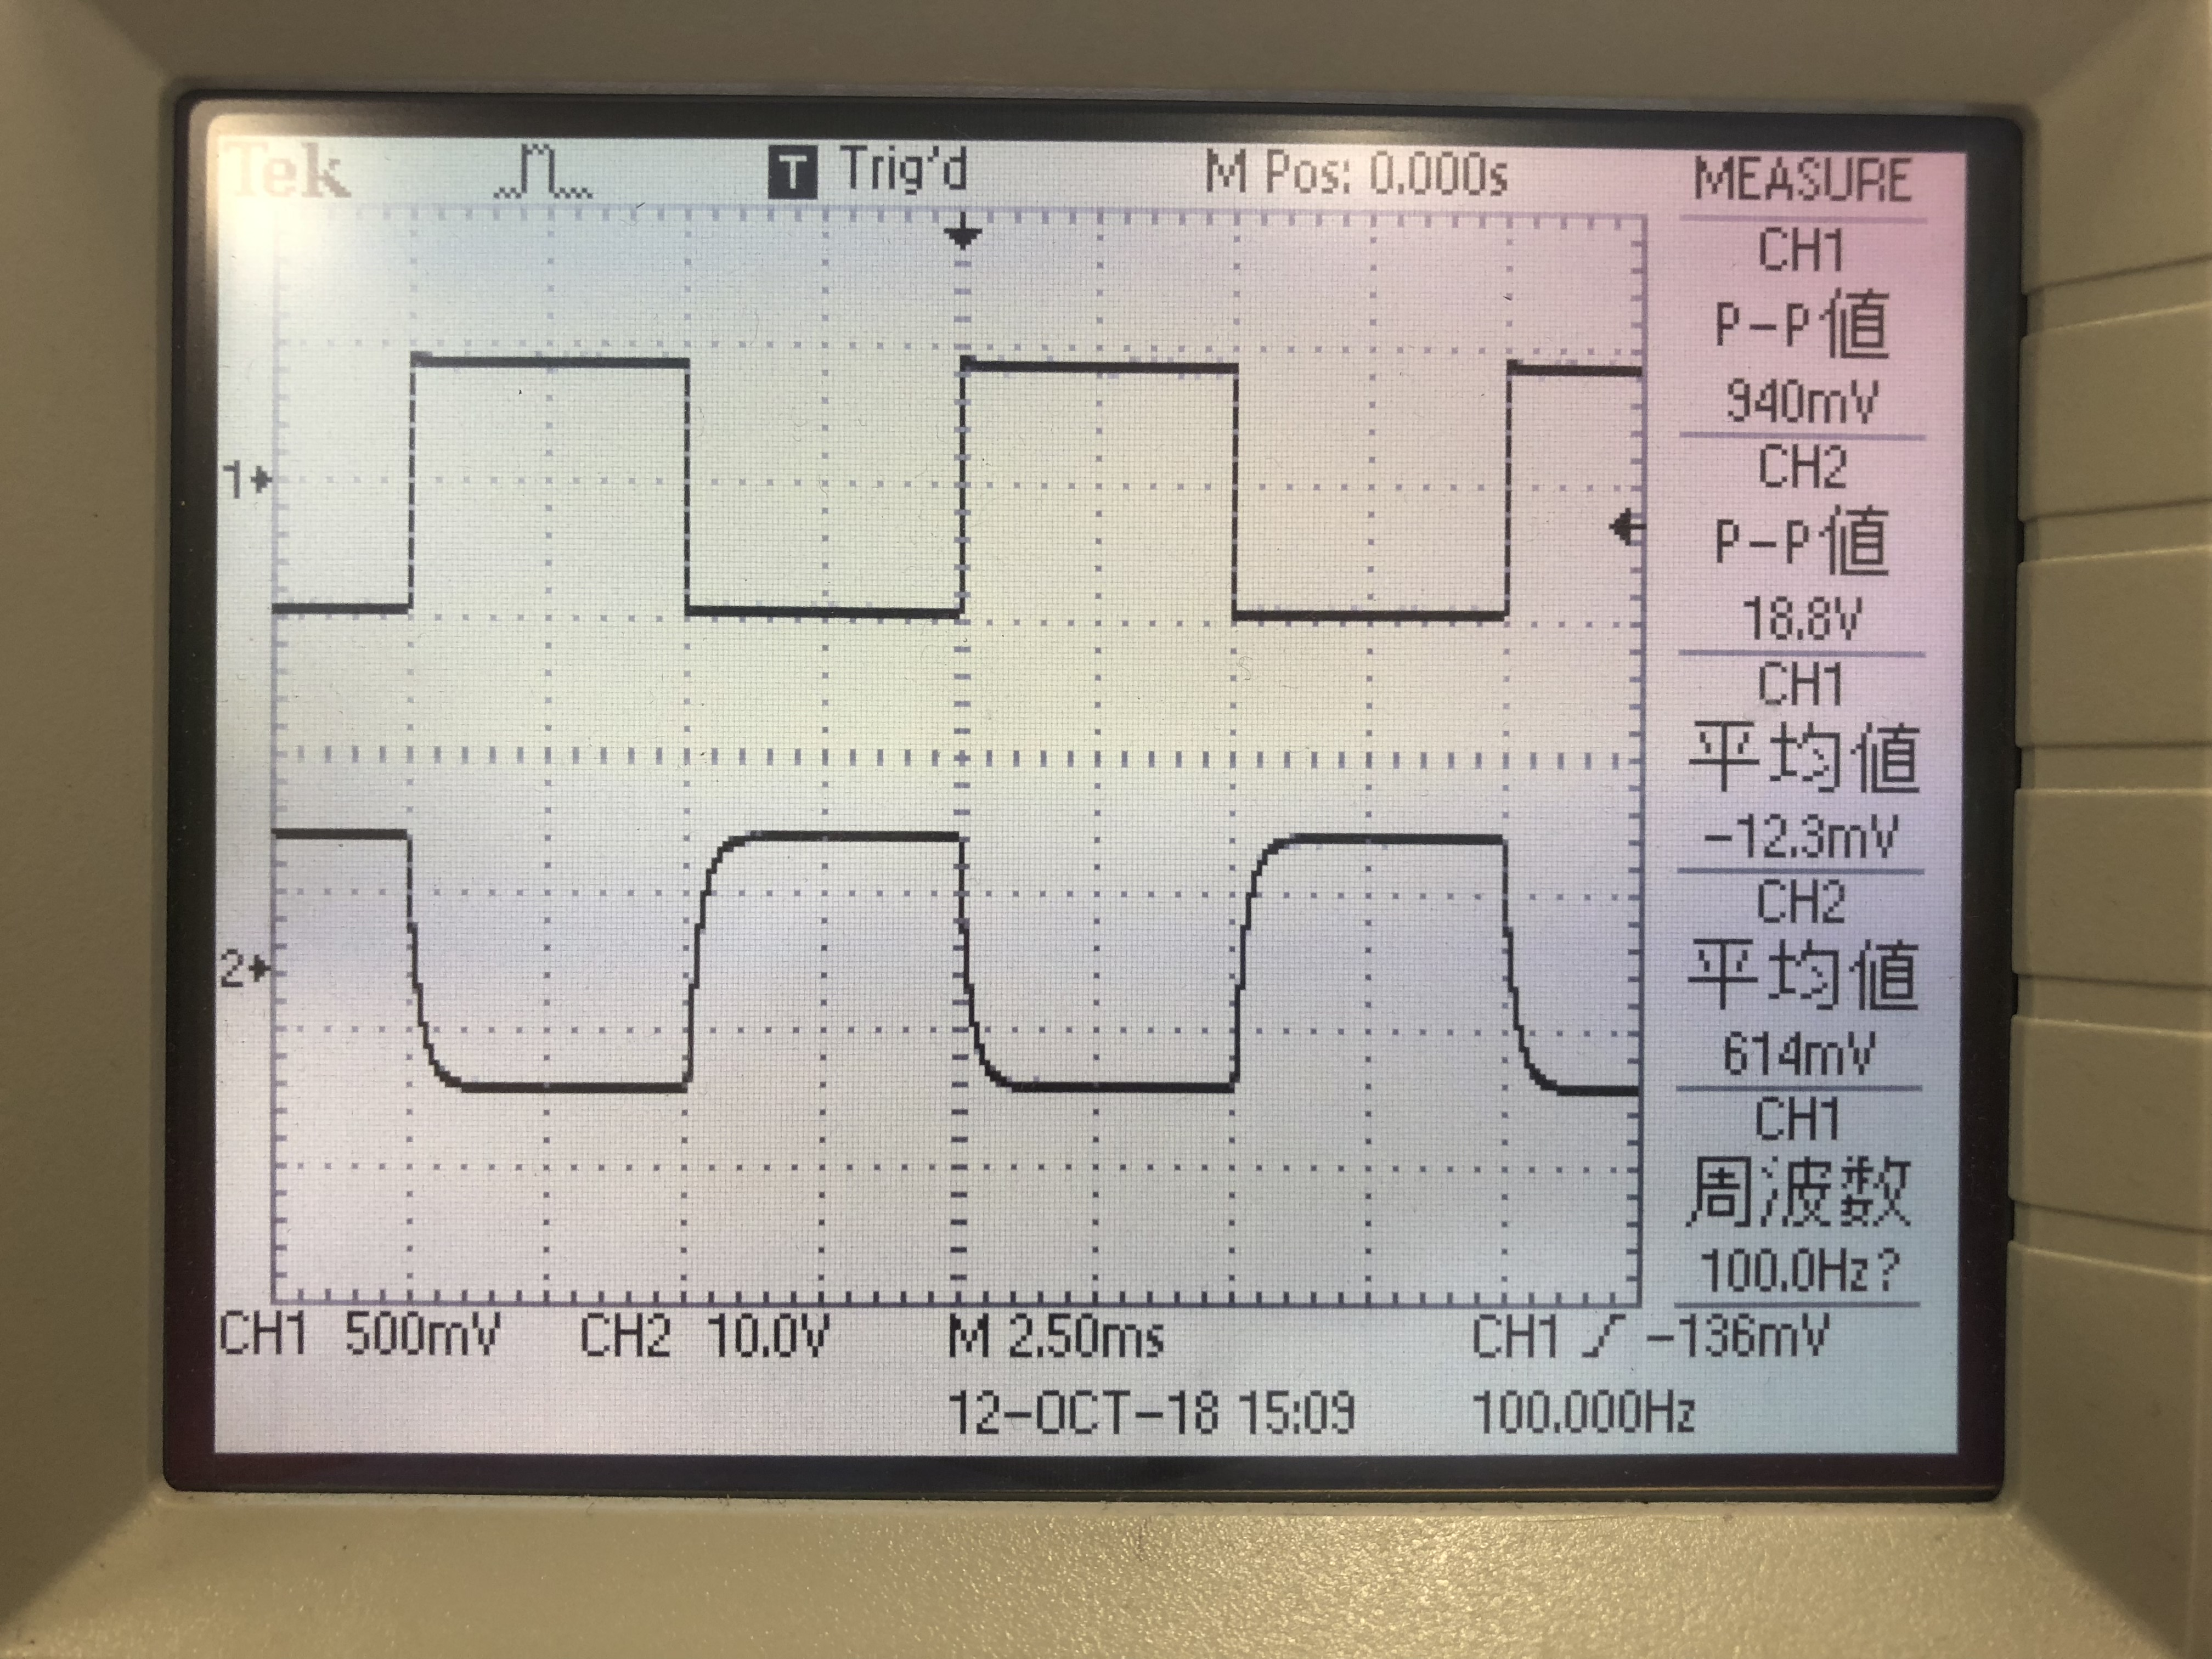
\includegraphics[width=8cm]{画像/f<fp.jpg}
		\caption{積分回路の出力波形($f<f_p$の時)}
	\end{center}
\end{figure}


\section{考察}
\subsection{反転増幅回路の理論増幅度と実測値との比較}
まず$A = -1$の時について考える.入力電圧と出力電圧の比の平均をとると,$-0.663$となった.
この時, 測定振れの大きい0V近傍については除いて計算した.つまり、理論増幅値と比べると実測値は$43.7\%$小さくなってしまったことになる。
これは外部に存在する電磁波によるノイズから生じる誤差, または回路の錆びや劣化によって計算値通りの性能を発揮できていないことが原因と考えられる。
次に$A = -10$の時についても考えてみる。入出力電圧比の平均は同様に計算すると$-9.534$となった。この時,  測定振れの大きい0V近傍と出力電圧比が一定な部分は除外した.
実測値は理論値と比べて$4.66\%$小さくなっている。$A=-1$の場合よりも$A=-10$の場合の方が増幅性能が上昇していることがわかる.
この理由としては、増幅度は$R_1$と$R_f$の比によって表されるため、$R_f$が大きい方が理論値の$A$と実測値の$A$の誤差が小さくなるため、また、
出力電圧が大きい方が出力電圧の振れによる読み取り誤差が小さいためであると思われる。
また$A=-10$の場合に入力電圧が約1.5V以上, また約-1.5V以下までは出力電圧が一定である理由としては、オペアンプの出力電圧範囲が15Vであるためであると思われる。

\subsection{反転増幅回路の動作周波数}
反転増幅回路の周波数特性と移送から、周波数が大きくなるにつれて電圧増幅度がなだらかに下がっていくことがわかった(図\ref{片対数1})。
入出力電圧の位相差[度]を見ると, 周波数が大きくなるのに追随して180度〜316.8度まで大きくなっている。
これはオペアンプのスルーレートによるものと考えられる。スルーレートとは、1$\mu$秒あたりに変化させられる電圧の限界値であり、
オペアンプによって固有のものである。スルーレートを超える時間あたりの電圧変化を生じさせようとすると波形が歪んでしまい、理想的な動作を行えなくなってしまう。
スルーレートは次式で表される。
\begin{align}
	SR = 2 \pi f V_{in}
\end{align}
今回使用した実習用オペアンプのスルーレートは公開されていないため正確な計算は行えないが、
急激に電圧増幅度が低下し始めている100〜200kHz付近が限界だとするとスルーレートの式より、
\begin{align}
	SR_min = 2 \times 3.14 \times (100 \times 10^3) \times 1.22 \times 10^{-6}= 0.766 [\mathrm{V/\mu s}] \\
	SR_Max = 2 \times 3.14 \times (200 \times 10^3) \times 1.22 \times 10^{-6}= 1.532 [\mathrm{V/\mu s}]
\end{align}
と求められ、実習用オペアンプのスルーレートは0.766〜1.532$\mathrm{V/\mu s}$であると推測することができる。
\subsection{反転・非反転増幅回路の特徴と相違点について}
反転増幅回路の特徴を列挙すると以下のものがある。
\begin{itemize}
	\item 入力に対して、出力が反転する。
	\item 減衰も可能。($R_f < R_1$ とすることで、増幅率が 1 より小さくなり、減衰動作となる。)
	\item 抵抗値の選定は、各部品の特性を元に決める。
  \item 仮想接地により、$V_{in}$側から見ると、$R_1$を介してGNDに接続している。電圧降下により、入力電圧が正しく伝わらない可能性がある。
	\item 回路の出力インピーダンスは、ほぼ 0。(負帰還により、出力電流が流れても、出力電圧は変化しない。つまり、出力電流が流れても、出力電圧の電圧降下はない。)
\end{itemize}

非反転増幅回路の特徴を列挙すると以下のものがある。
\begin{itemize}
	\item 入力に対して、出力が反転しない。
	\item 増幅率は1倍以上(減衰はできない)。($1 + \frac{R_f}{R_1}$にて、抵抗値が何であれ必ず1以上となる。)
	\item 入力電圧Vinが変動しても、負帰還により、変動に追従する。
	\item 回路の入力インピーダンスが極めて高いため(OPアンプの入力インピーダンスは非常に高く、入力電圧VinはOPアンプ直結)、信号源に不要な電圧降下を生じる心配がない。
	\item 回路の出力インピーダンスは、ほぼ 0。(負帰還により、出力電流が流れても、出力電圧は変化しない。つまり、出力電流が流れても、出力電圧の電圧降下はない。)
\end{itemize}

反転増幅回路では高い増幅度をを持つオペアンプに負帰還をかけ、増幅度を抑えて使うことで所望の増幅度の回路として使うことができる。
非反転増幅回路では, 入力と出力が反転しないため、位相が問題になる用途に用いられる。

\subsection{各フィルタの理論周波数特性($f-g$の関係)と実測周波数特性の比較及びカットオフ周波数について}
通過帯域と阻止帯域の境目となる周波数のことをカットオフ周波数または、遮断周波数という。
ローパスフィルタ回路、ハイパスフィルタ回路それぞれについて、式(\ref{式13}),(\ref{式14})を用いて、
理論値に基づいた$f−G$特性を示す片対数グラフを作成し、図\ref{ローパス比較},図\ref{ハイパス比較}として以下に示した。
このとき比較のために実測値のグラフも一緒に示した。

\begin{figure}[H]
  \begin{tabular}{cc}
    \begin{minipage}{0.5\hsize}
      \begin{center}
      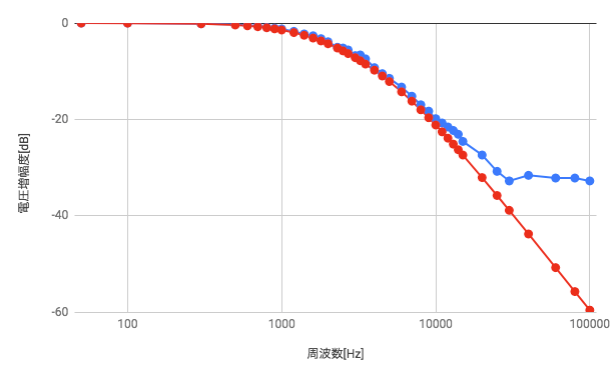
\includegraphics[width = 5cm]{画像/比較1.png}
      \caption{$f-G$特性の実測値と理論値の比較(ローパスフィルタ)}
      \label{ローパス比較}
      \end{center}
    \end{minipage}

    \begin{minipage}{0.5\hsize}
      \begin{center}
        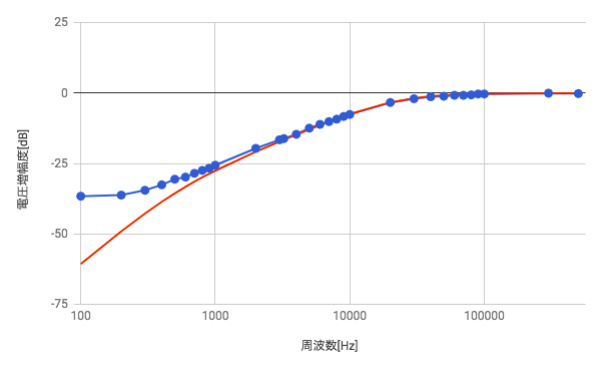
\includegraphics[width = 5cm]{画像/比較2.png}
        \caption{$f-G$特性の実測値と理論値の比較(ハイパスフィルタ)}
        \label{ハイパス比較}
      \end{center}
    \end{minipage}
  \end{tabular}
\end{figure}

ローパスフィルタ回路、ハイパスフィルタ回路ともに理論値の$f-G$特性と実測値は概ね沿っていることがわかる.
ローパスフィルタの高周波域(30000Hz以上)、ハイパスフィルタの低周波域(500Hz以下)では実測値が理論値を上回り、乖離してしまっている。
これは、減衰させた電圧が極小さな値に到達し、それ以上減衰させることが難しくなったためであると思われる。そのため、入力電圧をより上昇させて測定すれば
乖離はより遅れ、理論値により沿った実測値が得られると考えられる。

カットオフ周波数はローパスフィルタが1700Hz付近, ハイパスフィルタが20000Hz付近であると実測値から求められ、理論値においても同様の結果が得られた。
\subsection{微分・積分回路の動作周波数について}
微分回路では結果にある通り、周波数が大きくなるにつれ、上限値を境に微分機能が不安定になっている。
これはオペアンプの周波数特性によるものであり、高周波信号でゲインを大きくすると発振するという特性を持つためである。
積分回路では周波数が小さくなるにつれ、下限値を境に積分機能が不安定になっている。
これは低周波数では、オペアンプの増幅が有限であるために理想的な動作が行えなくなっている。

\section{感想}
電気回路についての知識と勉強不足を痛烈に感じた実験であった。この分野はあまり得意でなく、独学で掘り下げたこともほとんどなかったため、
授業の内容を上辺では理解していたものの、理論式を用いた証明や展開となると、繋がりや意味付けまでを理解しながら述べることは困難であった。
研究、就職と少なからずぶつかり学ばなければいけない分野であると思うので、なお一層のこと理解を深めていきたい。
\section{参考文献}
\\ \relax
[1]知能機械工学基礎実験,電気通信大学  知能機械工学科 \\ \relax
[2]ルネサスエレクトロニクスHPより https://www.renesas.com/jp/ja/support/technical-resources/engineer-school/electronic-circuits-03-op-amps-comparator-circuit.html\#op-amps-basics-1 \\ \relax
[3]マルツHP スルーレートとはより https://www.marutsu.co.jp/contents/shop/marutsu/mame/105.html

\end{document}
